% ==========================================================================================================
% DOCUMENT SETUP

\documentclass[12pt]{report}

% --- Packages ---
\usepackage[natbibapa]{apacite}  % APA 7 citations
\usepackage{enumitem}                    % bullet/numbered lists
\usepackage{amsmath, amssymb}           % math formatting and symbols
\usepackage{graphicx}                    % graphics/images inclusion
\usepackage{setspace}                    % line spacing
\usepackage{fontspec}                    % font customization
\usepackage{ragged2e}                    % text alignment
\usepackage{titlesec}                    % customize section/subsection
\usepackage{indentfirst}                 % indent first paragraph after headings
\usepackage{hyperref}                    % hyperlinks
\usepackage{pdflscape}                   % landscape pages
\usepackage[letterpaper, left=1.5in, right=1in, top=1in, bottom=1in, headheight=14.5pt]{geometry}
\usepackage{subcaption}
\usepackage{float}
\usepackage{tocloft}
\usepackage{etoolbox}


\usepackage[english]{babel}              % language hyphenation
\hyphenpenalty=1000
\tolerance=1000

\usepackage{chngcntr}                    % continuous equation numbering
\counterwithout{equation}{chapter}
% Display equation tags as "Equation (x)" on the right margin
\makeatletter
\renewcommand{\tagform@}[1]{\maketag@@@{Equation~(#1)\@@italiccorr}}
\makeatother

\usepackage{fancyhdr}                     % header/footer formatting
\fancypagestyle{plain}{
  \fancyhf{}
  \fancyhead[R]{\thepage}
  \renewcommand{\headrulewidth}{0pt}
}
\pagestyle{fancy}
\fancyhf{}
\fancyhead[R]{\thepage}
\renewcommand{\headrulewidth}{0pt}

\makeatletter
\pretocmd{\@chapter}{\thispagestyle{fancy}}{}{}
\makeatother

% Set font to Candara as stated in the STUDENT CAPSTONE/THESIS GUIDELINES 
\setmainfont{Candara}[Path=page/, Extension=.ttf,
    UprightFont = *,
    BoldFont = *b,
    ItalicFont = *i,
    BoldItalicFont = *z
]

% Figures Setup - Follows "Figure x (Bold) Desc (normal) 
\usepackage[labelfont=bf,labelsep=period]{caption}
\captionsetup[figure]{justification=centering}
\captionsetup[table]{justification=raggedright,singlelinecheck=false}
\renewcommand{\thefigure}{\thechapter-\arabic{figure}}
\renewcommand{\thetable}{\thechapter-\arabic{table}}
\renewcommand{\contentsname}{TABLE OF CONTENTS}
\renewcommand{\listfigurename}{LIST OF FIGURES}
\renewcommand{\listtablename}{LIST OF TABLES}
\renewcommand{\bibname}{REFERENCES}
\addto\captionsenglish{%
  \renewcommand{\contentsname}{TABLE OF CONTENTS}%
  \renewcommand{\listfigurename}{LIST OF FIGURES}%
  \renewcommand{\listtablename}{LIST OF TABLES}%
}
\setcounter{tocdepth}{2}
\setlength{\cftbeforetoctitleskip}{-1cm}
\setlength{\cftaftertoctitleskip}{36pt}
\setlength{\cftbeforeloftitleskip}{-1cm}
\setlength{\cftafterloftitleskip}{36pt}
\setlength{\cftbeforelottitleskip}{-1cm}
\setlength{\cftafterlottitleskip}{36pt}
\renewcommand{\cfttoctitlefont}{\hfill\bfseries\fontsize{14}{16}\selectfont}
\renewcommand{\cftaftertoctitle}{\hfill}
\renewcommand{\cftloftitlefont}{\hfill\bfseries\fontsize{14}{16}\selectfont}
\renewcommand{\cftafterloftitle}{\hfill}
\renewcommand{\cftlottitlefont}{\hfill\bfseries\fontsize{14}{16}\selectfont}
\renewcommand{\cftafterlottitle}{\hfill}
\renewcommand{\cftchapleader}{\cftdotfill{\cftdotsep}}
\renewcommand{\cftsecleader}{\cftdotfill{\cftdotsep}}
\renewcommand{\cftsubsecleader}{\cftdotfill{\cftdotsep}}
\renewcommand{\cftfigleader}{\cftdotfill{\cftdotsep}}
\renewcommand{\cfttableader}{\cftdotfill{\cftdotsep}}

% Set Line Spacing
\doublespacing

% Set Document Alignment
\justifying

% Set Paragraph indentation: 0.25 inch (7 spaces)
\setlength{\parindent}{0.25in}
\setlength{\parskip}{0pt}

% Chapter headings.
\titleformat{\chapter}[block]
  {\normalfont\bfseries\centering\fontsize{14}{16}\selectfont}
  {CHAPTER \thechapter}
  {0.5em}
  {\MakeUppercase}
\titlespacing{\chapter}{0pt}{-1cm}{36pt}
\titleformat{name=\chapter,numberless}[block]
  {\normalfont\bfseries\centering\fontsize{14}{16}\selectfont}
  {}
  {0pt}
  {\MakeUppercase}
\titlespacing{name=\chapter,numberless}{0pt}{-1cm}{36pt}

% Section headings.
\titleformat{\section}
  {\normalfont\bfseries\fontsize{13}{15}\selectfont}
  {\thesection}{1em}{}
\titlespacing{\section}{0pt}{24pt}{12pt}

% Subsection headings.
\titleformat{\subsection}
  {\normalfont\bfseries\fontsize{12}{14}\selectfont}
  {\thesubsection}{1em}{}
\titlespacing{\subsection}{0pt}{12pt}{6pt}

% ==========================================================================================================
% DOCUMENT CONTENT


\newcommand{\makethesistitlepage}[8]{%
  \begin{titlepage}
    \thispagestyle{empty}
    \singlespacing
    \normalfont\normalsize\bfseries
    \centering

    {#1 \par} % Thesis Title
    \vspace{6\baselineskip}

    {A #2 by \par} % Proposal Type
    \vspace{6\baselineskip}

    {\begin{tabular}{c}#3\end{tabular}\par} % Researchers Name(s)
    
    \vspace{6\baselineskip}

    {Submitted to the Department of #4 \par} % Researcher Department
    
    {College of #5 \par} % Researcher College
    
    {#6 \par} % Researcher University

    \vspace{6\baselineskip}

    {In Partial Fulfillment of the Requirements for the Degree \par}
    {Bachelor of Science in #7 \par} % Researcher Degree

    \vfill
    {#8 \par}
  \end{titlepage}
}


% Page Style
\doublespacing

\begin{document}

\pagestyle{fancy}
% Title Page
% \maketitle
\makethesistitlepage
  {FeatureSAGE: Stable Attribute Group Editing With Integrated StyleFeatureEditor Encoder for Enhanced Few-shot Image Generation}
  {Thesis}
  {Joshua Libando\\Sam Joash V. Antonio}
  {Computer Science}
  {Computing and Information Sciences (CCIS)}
  {Caraga State University -- Main Campus}
  {Computer Science (BSCS)}
  {\textbf{May 2026}}
\thispagestyle{empty}
\clearpage
% Preliminary Pages

% Approval Sheet

\pagenumbering{roman}
\setcounter{page}{2}

\chapter*{APPROVAL SHEET} 
\addcontentsline{toc}{chapter}{APPROVAL SHEET}

\begin{center}
This thesis entitled \textbf{FeatureSAGE: Stable Attribute Group Editing With Integrated StyleFeatureEditor Encoder for Enhanced Few-shot Image Generation}
prepared and submitted by \textbf{Joshua Libando} and \textbf{Sam Joash V. Antonio}
in partial fulfillment of the requirements for the degree \textbf{Bachelor of Science in Computer Science} is hereby accepted.
\end{center}

\vspace{1.5cm} % space before signatures

\begin{center}
\textbf{REGIEN B. NAKAZATO, MSc.} \\
Thesis Adviser
\end{center}

\vspace{0.8cm}

\begin{center}
\textbf{LUISITO L. TABADA, PhD} \\
Chair, Oral Examination Panel
\end{center}

\vspace{0.8cm}

\begin{minipage}[t]{0.45\textwidth}
\begin{center}
\textbf{MARIA BESA JOY ORTUYO, MSc.} \\
Panel Member
\end{center}
\end{minipage}%
\hfill
\begin{minipage}[t]{0.45\textwidth}
\begin{center}
\textbf{JOHN MICHAEL F. CUTAMORA} \\
Panel Member
\end{center}
\end{minipage}

\vspace{0.8cm}

\begin{center}
Accepted and approved for the conferral of the degree \textbf{Bachelor of Science in Computer Science}
in the 1\textsuperscript{st} semester of SY 2024-2025
\end{center}

\vspace{1cm}

\begin{flushright}
\textbf{JAYMER M. JAYOMA, ITD} \\
Dean, CCIS
\end{flushright}


% Dedication ==============================================================================================
\chapter*{DEDICATION}
\addcontentsline{toc}{chapter}{DEDICATION}

To God Almighty, for His boundless grace and wisdom that guided us through
this journey.

To our families, whose unwavering love, sacrifices, and belief in us made
this work possible.

To our community at Caraga State University, for fostering an environment
where curiosity and innovation thrive.


% Acknowledgments =========================================================================================
\chapter*{ACKNOWLEDGMENT}
\addcontentsline{toc}{chapter}{ACKNOWLEDGMENT}

We would like to express our deepest gratitude to all those who contributed to the successful 
completion of this thesis.

We extend our sincere appreciation to our thesis adviser, \textbf{Ms. Regien B. Nakazato, MSc.}, 
for her unwavering support, guidance, and encouragement throughout this research journey. 
Her invaluable insights and dedication have been instrumental in shaping this work.

We are profoundly grateful to \textbf{Dr. Bartosz Majcher, PhD}, for his exceptional assistance with
formatting, meticulous proofreading, and invaluable advice that helped refine this paper.
His expertise and generosity with his time significantly elevated the quality of this research.

Special thanks are extended to \textbf{Mr. John Carlo Tecson} and \textbf{Mr. Jeff Rio Mausisa} 
for graciously lending their computers and laptops during the hardware testing phase.
Their contribution was essential in enabling comprehensive experiments across diverse
hardware configurations, making this study possible.

We also acknowledge the \textbf{Department of Computer Science} and the
\textbf{College of Computing and Information Sciences (CCIS)} at Caraga State University
for providing the resources and academic environment that fostered this research.

Finally, we express our heartfelt gratitude to our families and friends for their constant
encouragement, patience, and understanding throughout this challenging but rewarding
academic endeavor.



% Main Content
\begin{doublespacing}
\tableofcontents
\end{doublespacing}
\clearpage
\addcontentsline{toc}{chapter}{LIST OF FIGURES}
\begin{doublespacing}
\listoffigures
\end{doublespacing}
\clearpage
\addcontentsline{toc}{chapter}{LIST OF TABLES}
\begin{doublespacing}
\listoftables
\end{doublespacing}

Few-shot image generation remains difficult because limited examples can cause mode collapse, reduced image quality, and unstable semantic edits. Stable Attribute Group Editing (SAGE) improves latent attribute editing for this setting, but its pixel2style2pixel (pSp) inversion path can lose local details and produce less reliable latent codes. This study proposes FeatureSAGE, a SAGE-based framework that integrates the StyleFeatureEditor Inverter and Feature Editor to represent images with both $W^{+}$ latent codes and intermediate feature tensors. The pretrained StyleGAN2 generator is kept fixed while feature-level editing is added to improve reconstruction detail and class-consistent variation. In one-shot experiments on FUNIT Animal Faces and 102 Flowers at 1024$\times$1024 resolution, FeatureSAGE achieves FID scores of 45.60 and 49.60, outperforming SAGE and AGE while maintaining comparable LPIPS on Flowers and Animal Faces, respectively. These results indicate that joint latent-feature inversion and editing improve few-shot attribute group editing without removing useful perceptual variation.


% Switch to Arabic numerals for chapters
\clearpage
\pagenumbering{arabic}

\section{Introduction}

Generative Adversarial Networks (GANs) learn an adversarial game between a generator and discriminator and have become a standard foundation for high-fidelity synthesis \cite{GAN}. StyleGAN and StyleGAN2 further improved image quality by mapping an input latent code into an intermediate style space and modulating synthesis layers, making semantic manipulation more practical than in the original latent space \cite{karras2019stylebasedgeneratorarchitecturegenerative,karras2020analyzingimprovingimagequality}. These properties are useful for few-shot image generation, where a model must synthesize plausible samples for a novel category from very limited references rather than retraining a generator from scratch.

Latent editing methods exploit the observation that many attributes correspond to directions or subspaces in StyleGAN representations \cite{shen2020interpretinglatentspacegans,harkonen2020ganspacediscoveringinterpretablegan}. Attribute Group Editing (AGE) applies this idea to few-shot generation by separating category-relevant class structure from category-irrelevant variations such as color, pose, and texture \cite{AGE}. Stable Attribute Group Editing (SAGE) improves AGE by estimating a more stable class embedding from few-shot examples and by adaptively selecting compatible attribute directions from related seen classes \cite{ding2023stableattributegroupediting}. However, SAGE still depends on a pSp inversion path, and encoder-based inversion can trade reconstruction fidelity against editability \cite{richardson2021encodingstylestyleganencoder,liu2023delvingstyleganinversionimage}.

This study addresses that limitation by integrating the StyleFeatureEditor (SFE) Inverter and Feature Editor into SAGE. Instead of representing an input only through $W^{+}$ style codes, FeatureSAGE predicts both a $W^{+}$ latent and an intermediate feature tensor, then edits both during synthesis \cite{bobkov2024devildetailsstylefeatureeditordetailrich}. The research problem is whether this feature-level inversion path can improve detail preservation, edit stability, and distributional quality for novel classes while retaining the SAGE mechanism for class-consistent few-shot attribute group editing.

Specifically, the study asks whether replacing pSp with SFE improves inversion fidelity and image-detail preservation, whether the change affects consistency and diversity for unseen Flowers and Animal Faces classes, and how the proposed framework compares with AGE and SAGE in image quality and edit reliability. These questions are important because few-shot augmentation is useful only when generated samples preserve category identity while still providing realistic non-category variation. A generator that produces visually plausible but class-inconsistent images can reduce downstream value, while a model that preserves the reference too closely may fail to provide useful diversity.

The practical motivation is data-efficient image synthesis for fine-grained domains where collecting many labeled examples is difficult. Animal-face and flower categories contain meaningful intra-class variation in color, texture, orientation, and local structure, but they also require strong preservation of category-specific appearance. This makes them suitable testbeds for evaluating whether a few-shot generator can introduce useful variation without corrupting the class-defining features of the reference image.

The contributions of this paper are as follows: (1) a FeatureSAGE framework that replaces the pSp-based SAGE inversion path with a StyleFeatureEditor Inverter and Feature Editor; (2) a one-shot evaluation protocol on FUNIT Animal Faces and 102 Flowers using the same pretrained StyleGAN2 setting, data splits, and metrics across AGE, SAGE, and FeatureSAGE; and (3) quantitative and qualitative evidence showing that FeatureSAGE lowers FID while keeping LPIPS close to the baselines. The study is limited to StyleGAN2-based few-shot image generation on Animal Faces and Flowers and does not evaluate optimization-based inversion or non-StyleGAN generators.

\section{Review of Related Literature}

\subsection{StyleGAN Latent Editing and Inversion}

StyleGAN introduced a style-based generator in which an input latent is transformed into an intermediate $W$ space and injected into synthesis layers, yielding stronger disentanglement and image quality than earlier GAN designs \cite{karras2019stylebasedgeneratorarchitecturegenerative}. StyleGAN2 improved this generator by replacing AdaIN with weight modulation and demodulation and by regularizing the latent-to-image mapping, which supports higher fidelity and more stable inversion \cite{karras2020analyzingimprovingimagequality}. These architectures enable latent traversal, where an image can be edited by adding an attribute direction to a latent code. Methods such as InterFaceGAN, GANSpace, and SeFa show that pose, color, expression, and other attributes can often be controlled through approximately linear directions in StyleGAN spaces \cite{shen2020interpretinglatentspacegans,harkonen2020ganspacediscoveringinterpretablegan,shen2021closedformfactorizationlatentsemantics}.

The latent representation chosen for editing strongly affects the balance between detail and control. A compact $W$ code tends to stay closer to the generator distribution and supports smoother edits, while $W^{+}$ assigns a separate style vector to each synthesis layer and improves reconstruction at the risk of less predictable edits. Feature-space representations can retain still finer spatial information, but they require an editing mechanism that does not simply overwrite details during synthesis. This tradeoff is central to FeatureSAGE because few-shot generation needs both stable class-level edits and preservation of local cues such as flower petal structure or animal-face texture.

For real images, latent editing first requires GAN inversion. Encoder-based methods such as pSp, e4e, and ReStyle predict $W^{+}$ codes efficiently, while optimization-based methods can improve reconstruction at the cost of speed \cite{richardson2021encodingstylestyleganencoder,tov2021designingencoderstyleganimage,alaluf2021restyleresidualbasedstyleganencoder}. The central difficulty is the fidelity-editability tradeoff: high-capacity inversions in $W^{+}$ can preserve fine detail, but may move codes away from regions where semantic edits remain reliable \cite{liu2023delvingstyleganinversionimage}. StyleFeatureEditor addresses this limitation by predicting both a $W^{+}$ latent and an intermediate feature tensor, then training a Feature Editor to update feature maps during editing \cite{bobkov2024devildetailsstylefeatureeditordetailrich}. This motivates its integration into SAGE, whose baseline pSp inversion may lose local information that is useful for class-consistent attribute editing.

This distinction matters because a few-shot image generator is not judged only by whether an edited output looks realistic in isolation. It must also preserve the category cues that make the single reference useful. If inversion discards local structure before the edit is applied, the downstream attribute editing stage cannot recover those details reliably. Conversely, if the representation preserves details but becomes too entangled, edits may change category identity. FeatureSAGE is positioned between these needs by retaining SAGE's disentangled attribute dictionary while using SFE to carry additional feature-level evidence through the decoder.

\subsection{Few-Shot Attribute Group Editing}

Few-shot image generation seeks to synthesize diverse samples for a novel category from one or a few references. Directly adapting a powerful generator to a very small target set can overfit and reduce diversity, so many approaches transfer a pretrained generator and regularize adaptation through freezing, contrastive losses, or distance preservation \cite{mo2020freezediscriminatorsimplebaseline,ojha2021fewshotimagegenerationcrossdomain,zhao2023closerlookfewshotimage}. Editing-based methods avoid full retraining by reusing latent directions learned from seen categories.

AGE formulates a category as a combination of category-relevant structure and category-irrelevant attributes, learning a sparse dictionary of transferable directions and applying them to unseen-class embeddings \cite{AGE}. SAGE improves the stability of AGE by estimating a class embedding using all available few-shot references and by selecting attribute directions from similar seen categories, thereby reducing class-inconsistent edits \cite{ding2023stableattributegroupediting}. TAGE further studies trustworthy attribute group editing using codebooks and prompt-driven semantic modules \cite{zhang2024tagetrustworthyattributegroup}. These works show that latent attribute dictionaries can support few-shot synthesis without retraining the generator, but their effectiveness still depends on inversion quality and on preserving class identity under multi-attribute changes.

The present work therefore keeps the SAGE factorization and adaptive editing logic rather than introducing a new few-shot generator. Its modification is narrower: the inversion and decoding path is strengthened using SFE so that the latent edit is paired with an edited feature tensor. This scope preserves the original SAGE research line while testing whether the known reconstruction benefits of feature-level inversion translate to one-shot attribute group editing.

The related work also motivates the selected baselines. AGE is the direct attribute-group editing baseline because it demonstrates few-shot generation through category-relevant and category-irrelevant decomposition. SAGE is the stronger baseline because it stabilizes AGE using class embedding mapping and adaptive editing. Comparing FeatureSAGE against both methods isolates whether the proposed inversion and feature-editing path improves a mature editing-based pipeline rather than merely outperforming an older formulation.

\chapter[METHODOLOGY]{Methodology}

This chapter describes the methodological design used to develop and evaluate the proposed FeatureSAGE framework. It outlines the research design, system requirements, data preparation, model architecture, evaluation protocol, and expected outcomes that guide the experimental implementation.

\section{Research Design}

This study, ``FeatureSAGE: Stable Attribute Group Editing With Integrated StyleFeatureEditing Encoder for Enhanced Few-Shot Image Generation,'' 
adopts a quantitative experimental research design to evaluate improvements to the existing SAGE framework. In particular, the GAN inversion 
module of SAGE is modified by integrating the StyleFeatureEditor (SFE) inverter and its Feature Editor module. The modification is evaluated 
under a one-shot setting, where attribute manipulation is conditioned on a single reference image per test instance. Objective evaluation is 
performed using Fr\'echet Inception Distance (FID) and Learned Perceptual Image Patch Similarity (LPIPS), which measure distributional image 
quality and perceptual variation, respectively.

% =============================================================================
\subsection{Experimental Setup}

The experimental setup is designed to evaluate the effectiveness of the proposed FeatureSAGE framework in comparison 
to the existing SAGE method. The evaluation follows a quantitative experimental design that involves controlled 
changes to the inversion and feature-editing components and the measurement of model outputs using standardized metrics.

\begin{itemize}
    \item \textbf{Independent Variable:} The main experimental manipulation is the GAN inversion method. The baseline SAGE configuration uses the original pixel2style2pixel (pSp) encoder, whereas the proposed FeatureSAGE configuration integrates the StyleFeatureEditor inverter and Feature Editor module.

    \item \textbf{Dependent Variables:}
    To objectively evaluate the effectiveness of the GAN inversion and editing pipeline, the following metrics are employed:
    \begin{itemize}
        \item Reconstruction quality and generated-image distribution alignment, measured using Fr\'echet Inception Distance (FID).
        \item Perceptual similarity or perceptual diversity, depending on the evaluation context, measured using Learned Perceptual Image Patch Similarity (LPIPS).
    \end{itemize}

    \item \textbf{Controlled Variables}
    \begin{enumerate}
        \item \textbf{Generator Architecture:} A fixed, pretrained StyleGAN2 generator is used in both configurations for consistent image synthesis capability.
        \item \textbf{Training Dataset:} Both configurations use the same FUNIT Animal Faces and 102 Flowers datasets with the same preprocessing and seen/unseen class splits.
        \item \textbf{Evaluation Protocol:} The same unseen categories, one-shot support samples, query sets, and evaluation procedures are used for both configurations.
        \item \textbf{Loss Functions:} Reconstruction and editing losses are applied consistently within the corresponding training phases.
        \item \textbf{Optimization Settings:} Both configurations use the Adam optimizer and the fixed learning-rate settings specified in the training strategy.
        \item \textbf{Evaluation Metrics:} FID and LPIPS are computed using the same implementations and parameters.
        \item \textbf{Hardware and Software Environment:} All experiments are conducted using the same GPU-enabled PyTorch environment to avoid performance inconsistencies.
    \end{enumerate}

    \item \textbf{Experimental Conditions}
    
    Two experimental configurations are used:
    \begin{itemize}
        \item SAGE (Baseline): Employs the original pSp encoder with StyleGAN2.
        \item FeatureSAGE (Proposed): Integrates the StyleFeatureEditor inverter and Feature Editor.
    \end{itemize}
\end{itemize}

% =========================================================================================

\subsection{Hardware and System Requirements}

All experiments were conducted on a virtual machine instance with GPU pass-through hosted on institutional cloud infrastructure. The same hardware and software configuration was used for the baseline and proposed models so that performance differences could be attributed to the inversion and feature-editing components rather than to changes in the execution environment. Table~\ref{tab:hardware_system_requirements} summarizes the system requirements reported for the implementation.

\begin{table}[H]
\centering
\setlength{\tabcolsep}{8pt}
\begin{tabular}{|p{0.28\linewidth}|p{0.62\linewidth}|}
\hline
\textbf{Component} & \textbf{Specification} \\ \hline
CPU & QEMU Virtual CPU version 2.5+, 2 processors at 2.19 GHz \\ \hline
RAM & 32.0 GB \\ \hline
GPU & NVIDIA GRID V100D-32A, virtualized Tesla V100 with 16 GB HBM2 \\ \hline
Storage & Not specified in the source implementation notes; storage is required for the datasets, model checkpoints, and generated outputs. \\ \hline
Software and frameworks & PyTorch environment; pretrained StyleGAN2 generator; pSp encoder for the baseline and editing-pair generation; StyleFeatureEditor inverter and Feature Editor; MTCNN for animal-face cropping and alignment; Adam optimizer; mixed precision for Feature Editor training; FID and LPIPS metric implementations. \\ \hline
\end{tabular}
\caption{Hardware and system requirements used in the experimental setup.}
\label{tab:hardware_system_requirements}
\end{table}

The GPU specification is important because FeatureSAGE performs multiple generator passes and feature-tensor operations during inversion and editing. The use of mixed precision in the Feature Editor phase reduces memory pressure on the 16 GB V100 vGPU while preserving the same model configuration and reported evaluation protocol.

% =========================================================================================

\subsection{Few-Shot Experimental Setting}

In this study, the term \emph{few-shot} refers to the number of reference images available per target class used to construct 
class-level latent representations for attribute group editing and downstream evaluation. A \textbf{one-shot} setting utilizes a single reference image 
per target class, representing an extreme data-scarce scenario in which attribute editing and inversion must be performed with minimal visual 
information. This one-shot configuration is applied consistently across all datasets and experimental conditions for both the baseline SAGE 
and the proposed FeatureSAGE framework. By explicitly controlling the evaluation to a single reference image per class, the experimental 
protocol enables a systematic assessment of FeatureSAGE's robustness, stability, and generalization capability under severe data limitations. 
The few-shot constraint is applied during test-time adaptation and evaluation on unseen classes, while the StyleGAN2 generator and attribute 
directions are learned from seen-category data.


\subsection{Hardware and System Requirements}
\label{sec:hardware_system_requirements}

All experiments were conducted on a virtual machine instance with GPU pass-through hosted on institutional cloud infrastructure. The same hardware and software environment was used for the baseline and proposed configurations so that differences in FID and LPIPS could be attributed to the inversion and editing pipeline rather than to system-level variation.

\begin{itemize}
    \item \textbf{CPU:} QEMU Virtual CPU version 2.5+ with two processors operating at 2.19~GHz.
    \item \textbf{RAM:} 32.0~GB system memory.
    \item \textbf{GPU:} NVIDIA GRID V100D-32A, a virtualized Tesla V100 GPU with 16~GB HBM2 memory.
    \item \textbf{Storage:} The exact storage capacity was not specified in the implementation details. The environment must store the FUNIT Animal Faces and 102 Flowers datasets, pretrained StyleGAN2 generator checkpoints, pSp and StyleFeatureEditor checkpoints, generated images, and evaluation outputs.
    \item \textbf{Software environment:} The implementation used a PyTorch environment with a pretrained StyleGAN2 generator, the pSp encoder baseline, the StyleFeatureEditor Inverter and Feature Editor, MTCNN-based preprocessing for Animal Faces, Adam optimization, mixed-precision training, Inception-v3 features for FID, and deep network features for LPIPS. The operating system was not explicitly specified in the implementation details.
\end{itemize}

The 16~GB V100-class GPU is particularly important because FeatureSAGE performs multiple generator and inversion passes and injects intermediate feature tensors during synthesis. Mixed precision was enabled during Feature Editor training to reduce memory usage while preserving the same experimental protocol across comparisons.


\section{Data Preprocessing}


\subsection{Data Sources}

This research draws from a range of publicly available datasets with a varied scope of visuals such as animal faces and flowers. The datasets are popular for generating and attribute-editing applications because of their quality and well-labeled categories. For the purpose of this research's emphasis on few-shot image synthesis, only a minority of the images from each dataset are employed. Specifically, a minimal set of representative samples per class are sampled to replicate the few-shot learning situation. The datasets used are:

\begin{enumerate}
    \item \textbf{FUNIT Animal Faces Dataset}
    \begin{figure}[ht]
        \centering
        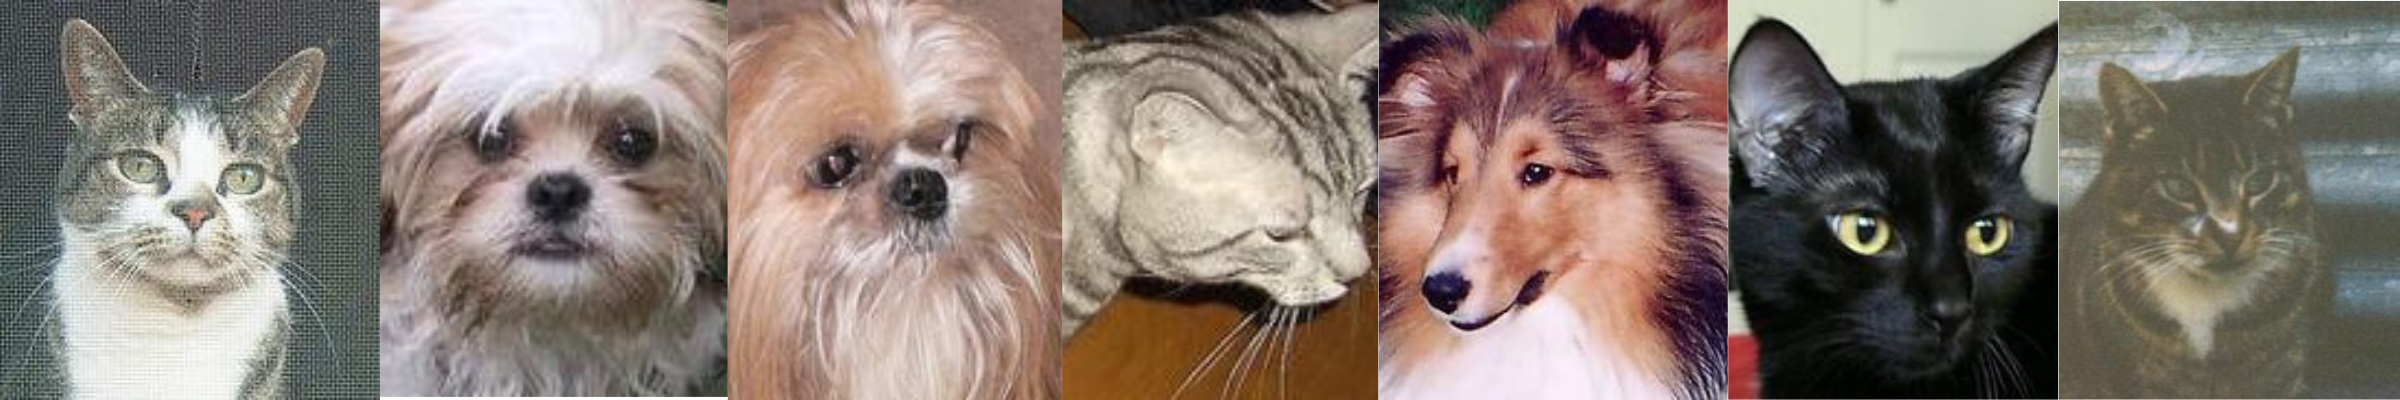
\includegraphics[width=0.9\linewidth]{images/funit_animal_faces_dataset.png}
        \caption{\textit{Sample images from the FUNIT Animal Faces dataset. Source: \citep{liu2019few}}}
        \label{fig:FUNIT_animal_faces}
    \end{figure}

    Figure~\ref{fig:FUNIT_animal_faces} shows representative samples from the FUNIT Animal Faces dataset. The dataset is comprised of 117,484 512~\(\times\)~512 
    resolution high-quality animal face images and is organized in 149 classes (each class is one animal species). Each domain includes a diverse range 
    of species and breeds, ensuring variation in appearance while maintaining consistent facial alignment to support generative model training. The images were 
    curated from openly available sources and standardized in resolution and alignment, with the eyes centrally positioned to provide consistency for learning. 
    A subset of the images is reserved as a test set, with the remainder used for training. The diversity and quality of the FUNIT Animal Faces dataset make it 
    a strong benchmark for generative and attribute-editing models in few-shot settings \citep{liu2019few}.

    \item \textbf{102 Flower (Flowers)}
    \begin{figure}[ht]
        \centering
        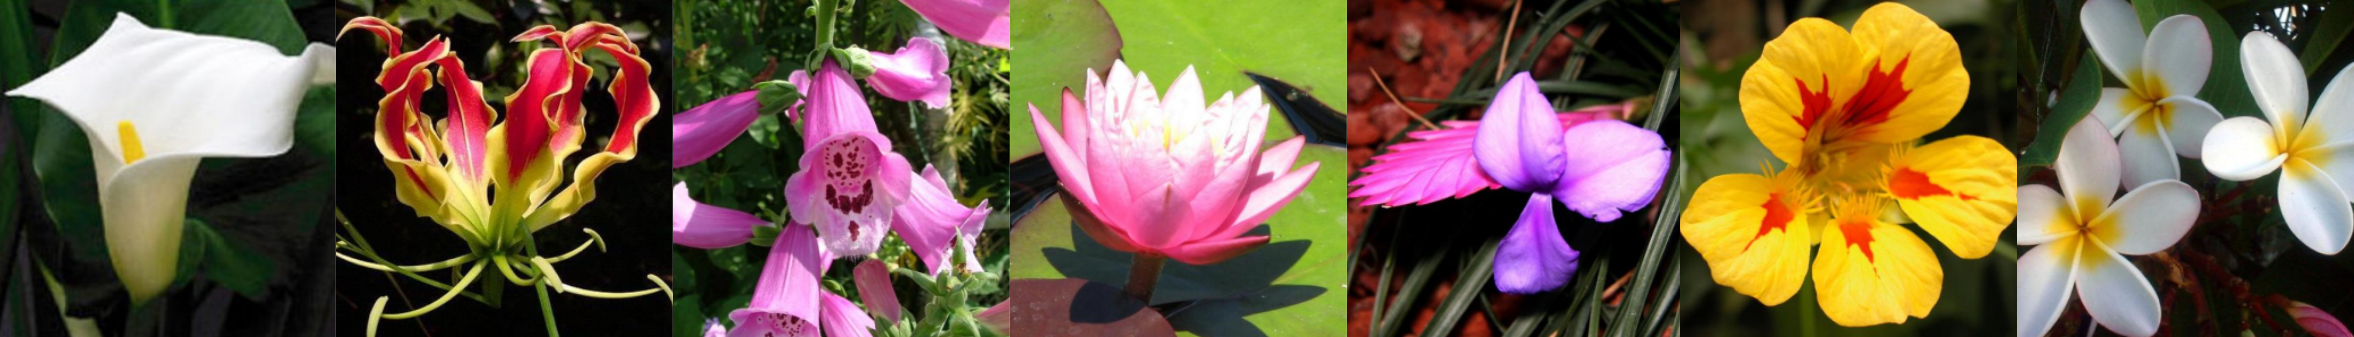
\includegraphics[width=0.9\linewidth]{images/flowers_dataset.png}
        \caption{\textit{Sample images from 102 Flower Dataset. Source \citep{Nilsback08}}}
        \label{fig:102Flower}
    \end{figure}

    Figure~\ref{fig:102Flower} shows sample images from the 102 Flower dataset, which comprises 102 flower classes present in the United Kingdom. There are between 40 and 258 images in each class. The flowers covered by the dataset are regularly occurring species in the UK. The dataset shows a great deal of variation in the sizes, pose, and lighting conditions of the flowers, which is an added complexity for the task of classification. Moreover, there are large intra-class differences for some categories, and there are many categories that are visually extremely similar to each other. All such attributes make the dataset extremely suitable for fine-grained visual categorization. The dataset was also used for analysis and visualization using isomap dimensionality reduction based on shape and color descriptors, which revealed the structure of the different flower categories. As for the sizes of the images, the raw images in the dataset are of varying sizes. For instance, one raw image from the dataset measures 500×667 pixels \citep{Nilsback08}.
    
\end{enumerate}

\subsection{Data Preprocessing Steps}

For all datasets, we will apply the following preprocessing steps:

\begin{itemize}
    \item Resizing and Normalization: Images will be resized to 256×256 for efficiency (and 512×512 for high-res experiments) and pixel values will be normalized to the range [-1,1] for input to StyleGAN2.
    \item Filtering: We will remove any extremely low-quality or mislabeled images.
    \begin{itemize}
        \item For FUNIT Animal Faces, use a face detector, MTCNN (Multi-Task Cascaded Convolutional Networks), to crop and horizontally align faces so the eyes are leveled.
    \end{itemize}

    \item Train-Test Splitting : We assess our approach on four standard few‐shot image domains, partitioning each into “seen” classes for model fitting and “unseen” classes for testing:
    
    \begin{itemize}
      \item \textbf{Animal Faces.} Out of the total categories, 120 are used as seen classes for training, while the remaining 30 serve as unseen classes for evaluation.
      \item \textbf{Flowers.} We assign 85 categories to the training (seen) split and reserve 15 categories for the test (unseen) split.
    \end{itemize}
    
    \item Augmentation: No data augmentation will be used beyond centering and flipping, since we focus on the evaluation of given domains. All datasets and preprocessing pipelines are documented for reproducibility.
\end{itemize}

\section{Model Architecture}

This study proposes a modified SAGE framework named \textbf{FeatureSAGE}. The architecture combines a pretrained StyleGAN2 generator, the StyleFeatureEditor inverter and Feature Editor, and SAGE's attribute group editing mechanism. The purpose of the modification is to improve the inversion stage of SAGE by representing each input image with both a layer-wise latent code and an intermediate feature tensor. This design follows the observation of \citet{ding2023stableattributegroupediting} that stronger inversion can further improve the potential of SAGE for generative augmentation, and it follows \citet{bobkov2024devildetailsstylefeatureeditordetailrich} in using both $W^+$ latents and feature latents for detail-preserving editing.

The main components of FeatureSAGE are:

\begin{enumerate}
    \item \textbf{StyleGAN2 generator:} The pretrained StyleGAN2 generator synthesizes images from latent codes. In FeatureSAGE, the generator receives the edited $W^+$ latent code together with an edited intermediate feature tensor produced by the Feature Editor.
    
    \item \textbf{StyleFeatureEditor inverter:} The inverter replaces the original pSp inversion module used in SAGE. For each input image, it predicts a $W^+$ latent code and an intermediate feature tensor. The $W^+$ code captures layer-wise style information, while the feature tensor carries spatial details that are difficult to preserve using latent codes alone.

    \item \textbf{Feature Editor:} The Feature Editor modifies the extracted feature tensor according to the latent-space edit. This allows the decoder path of the generator to synthesize images whose semantic edit is controlled by the latent code while finer details are supported by feature-level information.

    \item \textbf{SAGE attribute group editing:} The attribute factorization, class embedding mapping, and adaptive editing blocks are retained from SAGE. These blocks estimate category-relevant embeddings and category-irrelevant directions so that unseen classes can be edited under a one-shot setting.
\end{enumerate}

% ======================================================================================================

\subsection{Framework Overview}

\newgeometry{
    top=1cm,
    bottom=1cm,
    left=1cm,
    right=1cm
}

\begin{landscape}
    \begin{figure}[p]
        \centering
        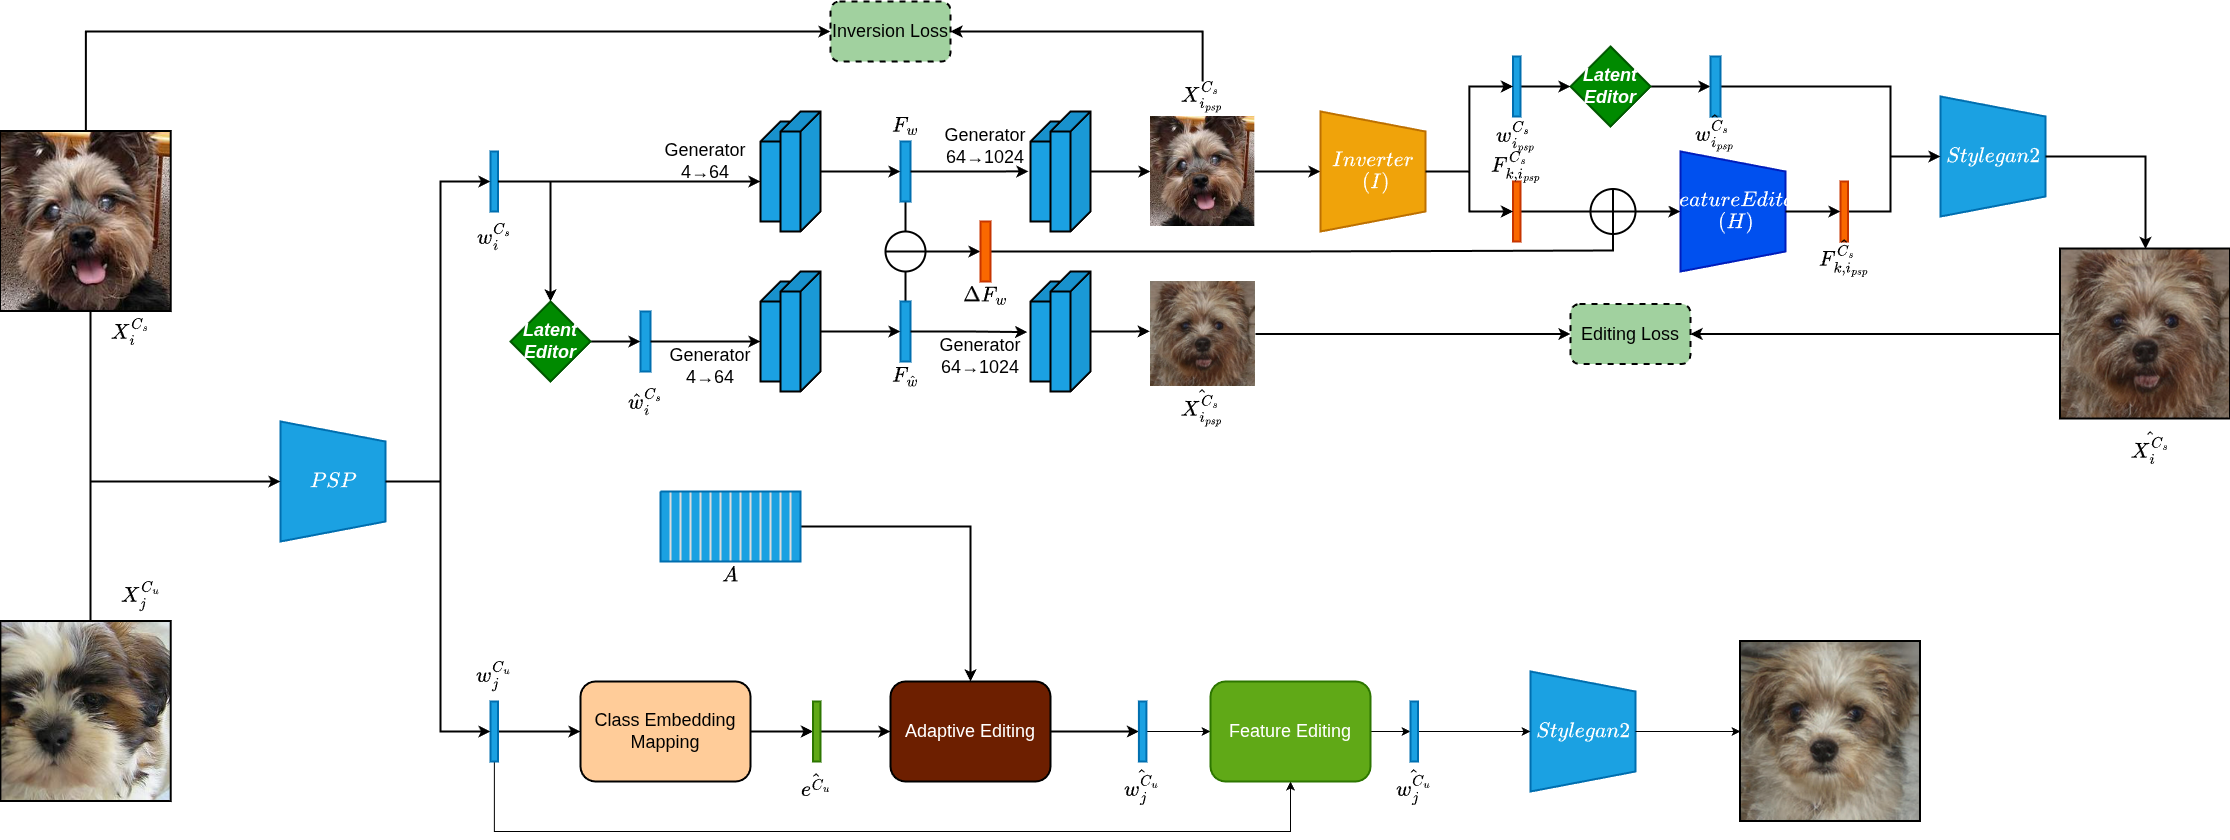
\includegraphics[
            width=\linewidth,
            height=\textheight,
            keepaspectratio
        ]{images/framework.png}
        \caption{FeatureSAGE framework}
        \label{fig:feature_sage_framework}
    \end{figure}
\end{landscape}

\restoregeometry

Figure~\ref{fig:feature_sage_framework} shows the overall FeatureSAGE framework. The training set for seen categories and the testing set for unseen categories are represented in Equation~\ref{eq:train-test-sets}:

\begin{equation}
D_{\mathrm{train}}=\{x_i^{C_s}\}_{i=1}^{N_s}, \qquad
D_{\mathrm{test}}=\{x_i^{C_u}\}_{i=1}^{N_u},
\label{eq:train-test-sets}
\end{equation}

where $x_i^{C_s}$ denotes an image from a seen category $C_s$, $x_i^{C_u}$ denotes an image from an unseen category $C_u$, and $N_s$ and $N_u$ denote the number of samples used from the seen and unseen splits, respectively. Equation~\ref{eq:train-test-sets} provides the notation used throughout the methodology for separating classes used in training from classes used during one-shot evaluation.

% ======================================================================================================

\subsection{Feature Extraction and Latent-Space Representation}

Feature extraction occurs before the generator synthesizes an output image. In the baseline SAGE configuration, the pSp encoder maps an input image into the extended StyleGAN2 latent space, as shown in Equation~\ref{eq:psp-inversion}:

\begin{equation}
PSP(x_i^{C_s}) = w_i^{C_s}, \qquad w_i^{C_s}\in W^+.
\label{eq:psp-inversion}
\end{equation}

In Equation~\ref{eq:psp-inversion}, $PSP(\cdot)$ is the pSp encoder and $w_i^{C_s}$ is the predicted $W^+$ latent code for a seen-category image. The $W^+$ space is important because it contains separate style vectors for the generator layers, allowing the model to represent coarse-to-fine visual attributes.

In FeatureSAGE, the StyleFeatureEditor inverter extracts two representations from an image, as defined in Equation~\ref{eq:sfe-inversion}:

\begin{equation}
I(x_i^{C}) = \left(w_i^{C}, F_{k,i}^{C}\right), \qquad
w_i^{C}\in W^+.
\label{eq:sfe-inversion}
\end{equation}

Here, $I(\cdot)$ is the StyleFeatureEditor inverter, $w_i^{C}$ is the layer-wise latent code, and $F_{k,i}^{C}$ is the intermediate feature tensor extracted at generator layer $k$. The document uses the ninth StyleGAN feature layer for feature injection. The latent code represents semantic and style-level information, while the feature tensor represents spatial detail and texture information. These two extracted features are significant because the latent code controls the edit direction, whereas the feature tensor helps preserve local details during synthesis.

The generator can also expose intermediate features for an original and edited latent code. Equation~\ref{eq:generator-feature-extraction} defines these generator-side features:

\begin{equation}
(x_{i,\mathrm{psp}}^{C_s},F_w)=G(w_i^{C_s}), \qquad
(\hat{x}_{i,\mathrm{psp}}^{C_s},F_{\hat{w}})=G(\hat{w}_i^{C_s}).
\label{eq:generator-feature-extraction}
\end{equation}

In Equation~\ref{eq:generator-feature-extraction}, $G(\cdot)$ is the StyleGAN2 generator, $F_w$ is the intermediate feature tensor associated with the original latent code, and $F_{\hat{w}}$ is the feature tensor associated with the edited latent code. These feature tensors are later used to compute the feature-space change required by the Feature Editor.

The latent space in FeatureSAGE therefore contains three related types of information: the $W^+$ latent code $w$, the category-level class embedding $e^C$, and the intermediate feature tensor $F_k$. The $W^+$ code encodes layer-wise style information; the class embedding stores category-relevant information through an average latent representation; and $F_k$ stores detail-rich spatial information used by the decoder block. Their combined use addresses the fidelity-editability trade-off identified in the literature without changing the reported experimental claims.

% ======================================================================================================

\subsection{Attribute Factorization}

\begin{figure}[ht]
    \centering
    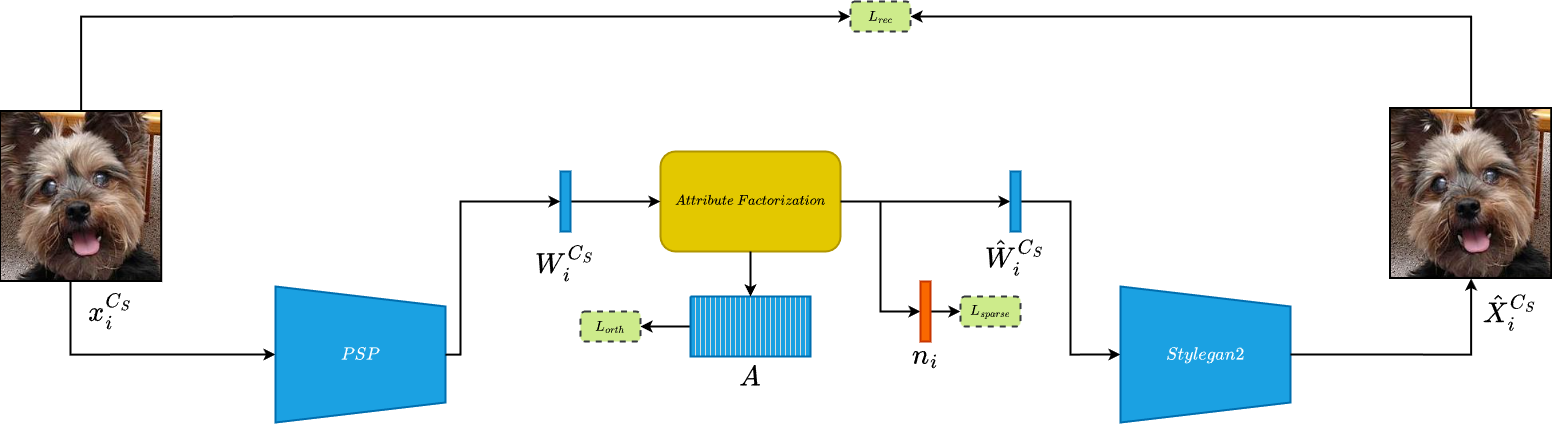
\includegraphics[width=1\linewidth]{images/SFSAGE.drawio.png}
    \caption{\textit{Attribute Factorization Training Framework \citep{ding2023stableattributegroupediting}}}
    \label{fig:attributge_fac_training}
\end{figure}

To enable disentangled editing, FeatureSAGE retains the SAGE attribute factorization block. The block learns category-irrelevant directions by comparing the latent code of a sample with the mean latent code of its category. The class embedding for a category is computed as the mean of its latent codes, as shown in Equation~\ref{eq:class-embedding}:

\begin{equation}
e^{C} = \frac{1}{N_C}\sum_{i=1}^{N_C} w_i^{C},
\label{eq:class-embedding}
\end{equation}

where $e^{C}$ is the class embedding for category $C$, $N_C$ is the number of latent codes available for the category, and $w_i^{C}$ is the latent code of the $i$th image. Equation~\ref{eq:class-embedding} provides the category-relevant center used to separate identity or class-level information from editable appearance variation.

\begin{figure}[ht]
    \centering
    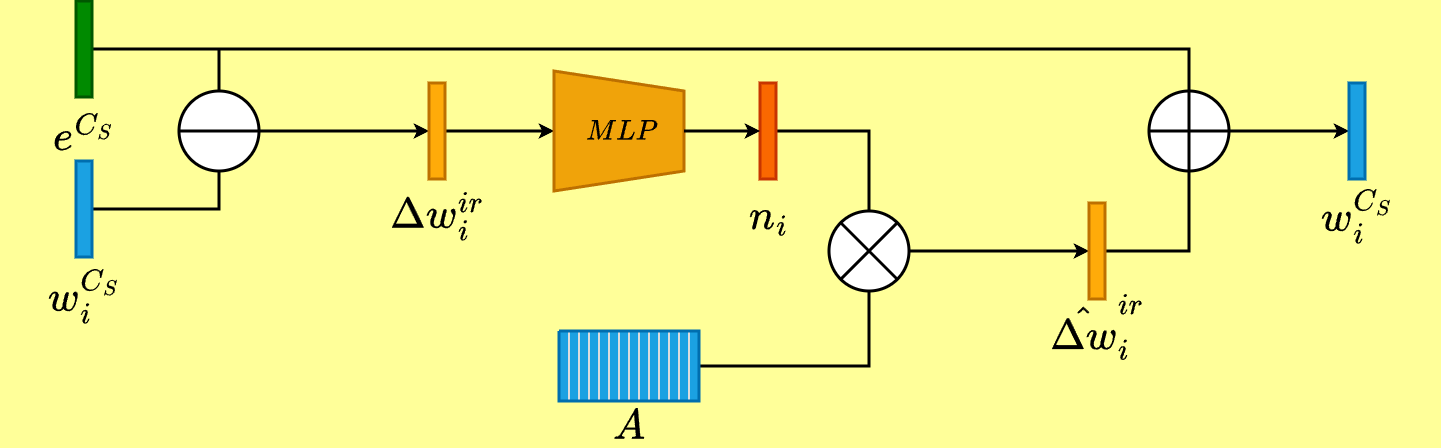
\includegraphics[width=1\linewidth]{images/AttributeFac.drawio.png}
    \caption{\textit{Attribute Factorization Block, derived from \citep{ding2023stableattributegroupediting}}}
    \label{fig:attribute_factorization_block}
\end{figure}

In the Attribute Factorization block shown in Figure~\ref{fig:attribute_factorization_block}, the category-irrelevant residual is computed in Equation~\ref{eq:category-irrelevant-residual}:

\begin{equation}
\Delta w_i^{ir}=w_i^{C_s}-e^{C_s}.
\label{eq:category-irrelevant-residual}
\end{equation}

In Equation~\ref{eq:category-irrelevant-residual}, $\Delta w_i^{ir}$ is the latent residual that remains after subtracting the class embedding $e^{C_s}$ from the sample latent code $w_i^{C_s}$. The purpose of this residual is to isolate appearance attributes that affect how an object looks without changing its class membership, such as orientation, color, background, texture, and expression.

The residual is then reconstructed using a learned sparse dictionary, as shown in Equation~\ref{eq:residual-factorization}:

\begin{equation}
\hat{\Delta w}_i^{ir}=A n_i.
\label{eq:residual-factorization}
\end{equation}

In Equation~\ref{eq:residual-factorization}, $A$ is the global dictionary of category-irrelevant directions and $n_i$ is the sparse coefficient vector predicted for the image. The dictionary basis follows sparse dictionary learning: each image is represented using only a small number of active directions so that individual directions remain more semantically interpretable.

Category-irrelevant editing is defined in Equation~\ref{eq:category-irrelevant-edit}. The edit changes appearance while preserving the category:

\begin{equation}
edit_{ir}(G(W_i^{C_s}))=
G\left(W_i^{C_s}+\alpha\Delta W^{ir},\,H(F_{k,i},\alpha\Delta W^{ir})\right)=\hat{X}_i^{C_s}.
\label{eq:category-irrelevant-edit}
\end{equation}

In Equation~\ref{eq:category-irrelevant-edit}, $edit_{ir}(\cdot)$ denotes category-irrelevant editing, $\alpha$ controls the edit intensity, $\Delta W^{ir}$ is the category-irrelevant direction, $H(\cdot)$ is the Feature Editor, and $\hat{X}_i^{C_s}$ is the edited image. The theoretical basis is the SAGE assumption that category-irrelevant directions can be learned from seen categories and transferred to unseen categories.

The sparse dictionary learning objective is stated in Equation~\ref{eq:sparse-dictionary-learning}:

\begin{equation}
\min_{n_i}\|n_i\|_0 \quad \mathrm{s.t.}\quad \Delta W_i^{ir}=A n_i.
\label{eq:sparse-dictionary-learning}
\end{equation}

In Equation~\ref{eq:sparse-dictionary-learning}, $\|n_i\|_0$ counts the number of nonzero entries in $n_i$. The purpose of the $L_0$ constraint is to encourage sparse use of the dictionary so that each generated edit is controlled by a limited number of directions.

In practice, SAGE optimizes this factorization with an encoder-decoder structure in which a Multi-Layer Perceptron (MLP) predicts the sparse representation, as shown in Equation~\ref{eq:mlp-sparse-code}:

\begin{equation}
n_i = MLP(\Delta W_i^{ir}).
\label{eq:mlp-sparse-code}
\end{equation}

Equation~\ref{eq:mlp-sparse-code} defines how the residual latent vector is encoded into the sparse coefficient vector used by the dictionary $A$.

% ======================================================================================================

\subsection{Class Embedding Mapping}

\begin{figure}[ht]
    \centering
    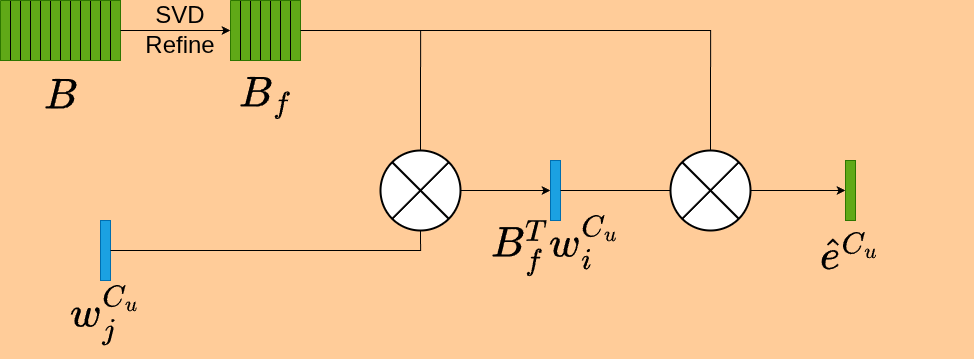
\includegraphics[width=1\linewidth]{images/Class_embedding_mapping.drawio.png}
    \caption{\textit{Class Embedding Block, adapted from \citep{ding2023stableattributegroupediting}}}
    \label{fig:class_embedding_block}
\end{figure}

Compared with Attribute Group Editing (AGE) \citep{AGE}, which randomly samples editing directions from $A$, SAGE uses class embedding mapping. The class embedding mapping block shown in Figure~\ref{fig:class_embedding_block} identifies the most important directions in the latent-code space for each category group and uses those directions to guide subsequent edits. This part of the framework remains unchanged in FeatureSAGE.

The class embedding set for the seen categories is denoted as $B$. Since the embeddings are computed from average latent codes, $B$ may still contain interference from category-irrelevant attributes. To filter the category-relevant subspace, singular value decomposition (SVD) is applied as shown in Equation~\ref{eq:svd-class-embedding}:

\begin{equation}
B = U_B \Sigma_B V_B^{T}.
\label{eq:svd-class-embedding}
\end{equation}

In Equation~\ref{eq:svd-class-embedding}, $B$ is the matrix of category-relevant class embeddings, $U_B$ contains the left singular vectors, $\Sigma_B$ contains singular values in descending order, and $V_B^{T}$ is the transpose of the right singular-vector matrix. The top-$t_B$ directions in $U_B$ are selected as the final category-relevant attribute dictionary $B_f \in \mathbb{R}^{18\times512\times t_B}$.

The class embedding of an unseen category is estimated using the filtered dictionary, as shown in Equation~\ref{eq:unseen-class-embedding}:

\begin{equation}
\hat{e}^{C_u} = \frac{1}{N_u}\sum_{i=1}^{N_u} B_f B_f^T W_i^{C_u}.
\label{eq:unseen-class-embedding}
\end{equation}

In Equation~\ref{eq:unseen-class-embedding}, $\hat{e}^{C_u}$ is the estimated embedding for unseen category $C_u$, $N_u$ is the number of latent codes available for that unseen category, and $W_i^{C_u}$ is the latent code of the $i$th unseen-category sample. The projection $B_fB_f^T W_i^{C_u}$ retains category-relevant components while suppressing most category-irrelevant variation.

% ======================================================================================================

\subsection{Adaptive Editing}

\begin{figure}[ht]
    \centering
    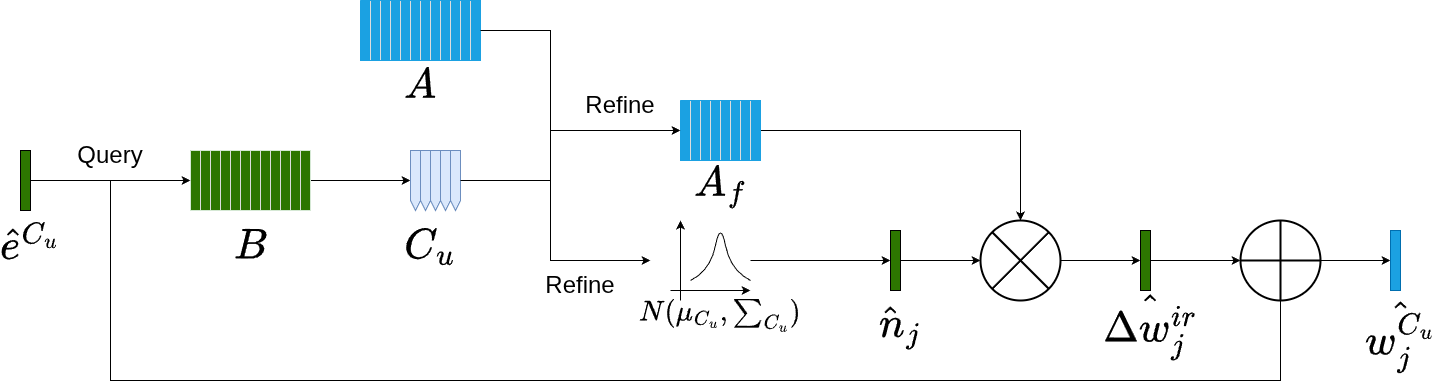
\includegraphics[width=1\linewidth]{images/adaptive.drawio.png}
    \caption{\textit{Adaptive Editing Block, from \citep{ding2023stableattributegroupediting}}}
    \label{fig:adaptive_editing_block}
\end{figure}

Figure~\ref{fig:adaptive_editing_block} shows the adaptive editing block of FeatureSAGE. Category-irrelevant qualities typically have similar distributions in closely related categories but may differ across distant categories. Therefore, adaptive editing selects seen categories that are close to an unseen category in the class-embedding space and uses their common editing directions to guide generation.

To identify the category-irrelevant editing directions that best fit an unseen category $C_u$, the residual direction is back-projected into the sparse representation, as shown in Equation~\ref{eq:back-projection}:

\begin{equation}
\hat{n}_i = A^{\dagger}\Delta W_i^{ir}.
\label{eq:back-projection}
\end{equation}

In Equation~\ref{eq:back-projection}, $A^{\dagger}$ denotes the pseudo-inverse of the dictionary $A$, $\Delta W_i^{ir}$ is the category-irrelevant residual, and $\hat{n}_i$ is the estimated sparse representation. The pseudo-inverse is used to express an observed residual in the coordinate system of the learned dictionary.

The mean absolute activation of sparse directions across the top-$t_C$ similar seen categories is computed in Equation~\ref{eq:mean-absolute-sparse-code}:

\begin{equation}
\overline{|n|}^{C_u} =
\frac{1}{t_C}\sum_{t=1}^{t_C}
\frac{1}{N_{S_t}}\sum_{i=1}^{N_{S_t}}
\left|\hat{n}_i^{C_{S_t}}\right|.
\label{eq:mean-absolute-sparse-code}
\end{equation}

In Equation~\ref{eq:mean-absolute-sparse-code}, $t_C$ is the number of similar seen categories, $N_{S_t}$ is the number of samples in the $t$th selected seen category, and $\hat{n}_i^{C_{S_t}}$ is the sparse representation of the $i$th sample from that category. The result $\overline{|n|}^{C_u}$ measures which dictionary directions are frequently or strongly activated for categories similar to $C_u$. For each layer in $W^+$, the top-$t_A$ directions are selected from $A$ to form the adaptive category-irrelevant dictionary $A_{C_u}\in\mathbb{R}^{18\times512\times t_A}$.

SAGE assumes that the sparse representations for related categories follow a Gaussian distribution. This distribution is estimated in Equation~\ref{eq:adaptive-gaussian}:

\begin{equation}
\tilde{n}_j \sim \mathcal{N}(\mu_{C_u},\Sigma_{C_u}).
\label{eq:adaptive-gaussian}
\end{equation}

In Equation~\ref{eq:adaptive-gaussian}, $\mu_{C_u}$ and $\Sigma_{C_u}$ are the estimated mean and covariance of sparse codes for the selected categories, and $\tilde{n}_j$ is a sampled sparse code used to generate a new image. This sampling step provides controlled diversity for the unseen category.

The final adaptive generation equation is given in Equation~\ref{eq:adaptive-generation}:

\begin{equation}
X_j^{C_u} =
G\left(\hat{e}^{C_u}+\alpha A_{C_u}\tilde{n}_j,\,
H(F_{k,j}^{C_u},\alpha A_{C_u}\tilde{n}_j)\right).
\label{eq:adaptive-generation}
\end{equation}

In Equation~\ref{eq:adaptive-generation}, $X_j^{C_u}$ is a generated image for unseen category $C_u$, $\hat{e}^{C_u}$ is the estimated class embedding, $A_{C_u}$ is the adaptive dictionary, $\tilde{n}_j$ is the sampled sparse code, $\alpha$ controls the strength of the edit, and $H(\cdot)$ edits the feature tensor used by the generator. This equation summarizes how FeatureSAGE transforms one-shot class information and sampled attribute variation into a generated image.

% ======================================================================================================

\subsection{Feature Editing Decoder Block}

\begin{figure}[ht]
    \centering
    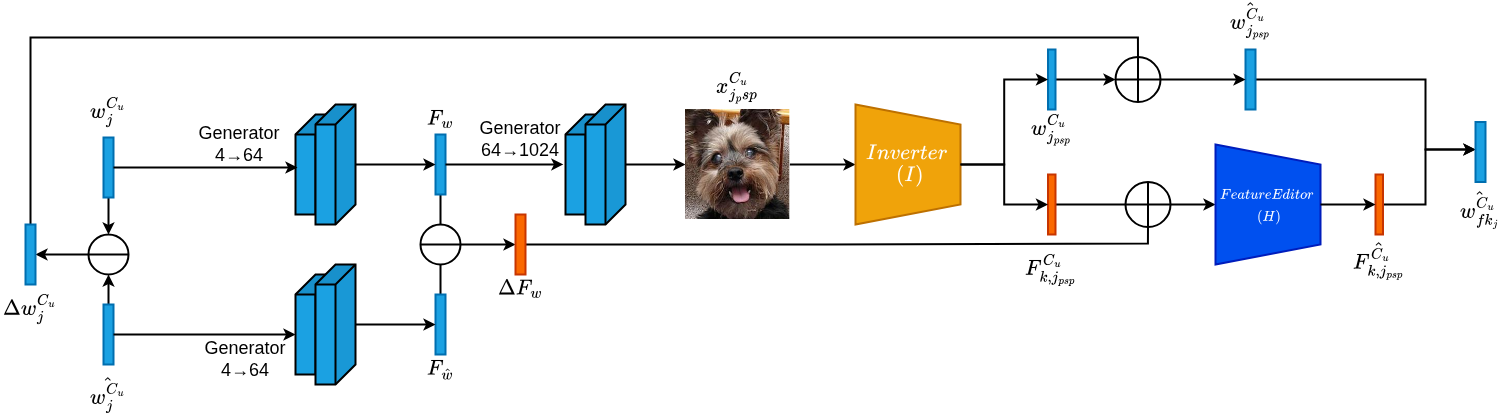
\includegraphics[width=1\linewidth]{images/featureEditordrawio.drawio.png}
    \caption{\textit{Feature Editing Decoder Block}}
    \label{fig:featureEditingBlock}
\end{figure}

Figure~\ref{fig:featureEditingBlock} shows the Feature Editing Decoder Block. The block receives the original latent representation, the edited latent representation produced by adaptive editing, and the intermediate feature tensor extracted by the StyleFeatureEditor inverter. Its role is to transform the input features into an edited feature tensor that can be injected into the ninth StyleGAN feature layer during image synthesis.

The latent-space difference used to describe the semantic edit is defined in Equation~\ref{eq:latent-difference}:

\begin{equation}
\Delta w_j^{C_u}=\hat{w}_j^{C_u}-w_j^{C_u}.
\label{eq:latent-difference}
\end{equation}

In Equation~\ref{eq:latent-difference}, $w_j^{C_u}$ is the original latent code and $\hat{w}_j^{C_u}$ is the edited latent code. This difference specifies the semantic movement applied in $W^+$.

The feature-space difference used for feature injection is defined in Equation~\ref{eq:feature-difference}:

\begin{equation}
\Delta F_w = F_w - F_{\hat{w}}.
\label{eq:feature-difference}
\end{equation}

In Equation~\ref{eq:feature-difference}, $F_w$ is the intermediate feature tensor produced from the original latent code and $F_{\hat{w}}$ is the corresponding tensor produced from the edited latent code. The decoder block uses this difference to determine how the original feature tensor should be modified to match the target semantic edit.

The Feature Editor transformation is represented in Equation~\ref{eq:feature-editor-transform}:

\begin{equation}
F_{k,j}^{\mathrm{edit}} = H(F_{k,j}^{C_u}, \Delta F_w).
\label{eq:feature-editor-transform}
\end{equation}

In Equation~\ref{eq:feature-editor-transform}, $F_{k,j}^{C_u}$ is the feature tensor extracted by the inverter for the unseen-category input, $\Delta F_w$ is the feature difference from Equation~\ref{eq:feature-difference}, and $F_{k,j}^{\mathrm{edit}}$ is the edited tensor injected into the generator. The decoder therefore modifies the feature-level representation while the edited latent code controls the global semantic direction. The output image is then synthesized by the generator using the edited latent code and the edited feature tensor, as shown in Equation~\ref{eq:decoder-synthesis}:

\begin{equation}
\hat{X}_j^{C_u}=G(\hat{w}_j^{C_u}, F_{k,j}^{\mathrm{edit}}).
\label{eq:decoder-synthesis}
\end{equation}

Equation~\ref{eq:decoder-synthesis} completes the decoder pathway: input image features and latent edits are transformed into an edited high-resolution output.

% ======================================================================================================
\subsection{Training Strategy}

In the training stage, a StyleGAN2 generator is trained using images from the seen categories. The StyleFeatureEditor inverter and the pSp encoder are also trained or used according to their roles in the pipeline. To manage resource consumption, FeatureSAGE uses a two-phase strategy: attribute factorization training followed by Feature Editor training.

\subsection{Phase 1: Attribute Factorization Training}

Phase 1 trains the attribute factorization block for disentangled sampling of category-irrelevant directions. The following losses are applied to the attribute factorization block.

\begin{itemize}
    \item \textbf{Sparsity Loss ($L_{\mathrm{sparse}}$):} The sparsity loss encourages the learned attribute code to activate only a small number of dictionary directions. Equation~\ref{eq:sparsity-loss} defines the loss:
    \begin{equation}
    L_{\mathrm{sparse}} = \left\|\sigma(\theta_0 n_i-\theta_1)\right\|_1.
    \label{eq:sparsity-loss}
    \end{equation}
    In Equation~\ref{eq:sparsity-loss}, $\sigma(\cdot)$ denotes the sigmoid function, $n_i$ is the sparse code, and $\theta_0$ and $\theta_1$ are hyperparameters controlling sparsity. The sigmoid compresses the MLP output and the $L_1$ norm approximates sparse behavior in a differentiable way.

    \item \textbf{Reconstruction Loss ($L_{\mathrm{rec}}$):} The reconstruction loss anchors the edited output to the input image so that edits do not destroy the original content. Equation~\ref{eq:reconstruction-loss} defines this loss:
    \begin{equation}
    L_{\mathrm{rec}}=\left\|G(e^{C_s}+A n_i)-x_i^{C_s}\right\|_2.
    \label{eq:reconstruction-loss}
    \end{equation}
    In Equation~\ref{eq:reconstruction-loss}, $e^{C_s}$ is the class-center latent, $A n_i$ is the attribute offset, $G(\cdot)$ is the generator, and $x_i^{C_s}$ is the input image. The loss penalizes large differences between the generated reconstruction and the original image.

    \item \textbf{Orthogonality Loss ($L_{\mathrm{orth}}$):} The orthogonality loss discourages category-irrelevant directions from overlapping with category-relevant directions. Equation~\ref{eq:orthogonality-loss} defines this loss:
    \begin{equation}
    L_{\mathrm{orth}}=\left\|B^T A\right\|_F^2.
    \label{eq:orthogonality-loss}
    \end{equation}
    In Equation~\ref{eq:orthogonality-loss}, $A$ is the category-irrelevant dictionary, $B$ is the category-relevant embedding basis, and $\|\cdot\|_F^2$ denotes the squared Frobenius norm. This term preserves class identity by reducing leakage between the category-relevant and category-irrelevant subspaces.
\end{itemize}

The overall attribute factorization loss is defined in Equation~\ref{eq:attribute-factorization-loss}:

\begin{equation}
L_{\mathrm{af}}=L_{\mathrm{rec}}+\lambda_1 L_{\mathrm{orth}}+\lambda_2 L_{\mathrm{sparse}}.
\label{eq:attribute-factorization-loss}
\end{equation}

In Equation~\ref{eq:attribute-factorization-loss}, $\lambda_1$ and $\lambda_2$ are weights for the orthogonality and sparsity losses \citep{ding2023stableattributegroupediting}. Training uses the Adam optimizer with a fixed learning rate of $1\times10^{-4}$, $\lambda_1=5\times10^{-4}$, $\lambda_2=5\times10^{-3}$, $\theta_0=5\times10^{-1}$, and $\theta_1=-1$.

\subsection{Phase 2: Feature Editor Training}

Phase 2 trains the Feature Editor $H$ using editing pairs generated with a pretrained pSp encoder. Following \citet{bobkov2024devildetailsstylefeatureeditordetailrich}, an input image $X$ is encoded into $w$, edited by a sampled direction from the adaptive editing procedure, and paired with the corresponding edited image $\hat{X}$. This trains $H$ to edit feature tensors according to the category-irrelevant attributes learned in Phase 1. To prevent the Feature Editor from relying only on synthetic editing pairs, it is also trained on the classical inversion task with $\Delta=0$.

The editing loss is defined in Equation~\ref{eq:feature-edit-loss}:

\begin{equation}
L_{\mathrm{edit}}(X,\hat{X}) =
\lambda_{l_2}\|X-\hat{X}\|_2+
\lambda_{\mathrm{lpips}}\mathcal{L}_{\mathrm{lpips}}(X,\hat{X}).
\label{eq:feature-edit-loss}
\end{equation}

The inversion loss uses the same reconstruction and perceptual terms, as shown in Equation~\ref{eq:feature-inversion-loss}:

\begin{equation}
L_{\mathrm{inv}}(X,\hat{X}) =
\lambda_{l_2}\|X-\hat{X}\|_2+
\lambda_{\mathrm{lpips}}\mathcal{L}_{\mathrm{lpips}}(X,\hat{X}).
\label{eq:feature-inversion-loss}
\end{equation}

Equations~\ref{eq:feature-edit-loss} and \ref{eq:feature-inversion-loss} use $L_2$ reconstruction and LPIPS perceptual losses to preserve both pixel-level structure and perceptual similarity. The total Feature Editor loss is defined in Equation~\ref{eq:feature-editor-loss}:

\begin{equation}
L_{\mathrm{fe}} = L_{\mathrm{edit}}(X,\hat{X}) + L_{\mathrm{inv}}(X,\hat{X}).
\label{eq:feature-editor-loss}
\end{equation}

In Equation~\ref{eq:feature-editor-loss}, the editing term teaches $H$ to respond to nonzero edit directions, while the inversion term with $\Delta=0$ stabilizes feature reconstruction. The Feature Editor is trained using the Adam optimizer with a fixed learning rate of $1\times10^{-4}$ for 15,000 iterations on a single V100 16 GB vGPU. Mixed precision is enabled to improve memory efficiency because the phase requires multiple generator passes. The loss weights are $\lambda_{l_2}=10$ and $\lambda_{\mathrm{lpips}}=0.8$, with an additional LPIPS scaling factor of 0.5. The sparse dictionary $A$ is initialized with a fixed length of 100.


\subsection{Evaluation Protocol}

% ===============================================================================
\subsubsection{Evaluation Metrics}

We evaluated the models using quantitative metrics for both reconstruction quality and editing performance, under a few-shot test-time setup.   

\begin{enumerate}
    \item \textbf{Fr\'echet Inception Distance (FID)}

    The Fr\'echet Inception Distance (FID) is a widely adopted metric for evaluating the quality of images generated by deep generative models, particularly in tasks such as few-shot image generation \cite{heusel2017gans, wang2023attribute}. Rather than comparing images directly at the pixel level, FID operates in a high-level feature space extracted from a pretrained Inception-v3 network \cite{heusel2017gans}. This makes it effective for capturing both the fidelity (realism) and diversity (variety) of generated samples \cite{borji2022pros}. The FID score is computed by modeling the feature distributions of real and generated images as multivariate Gaussians \cite{heusel2017gans}. The FID score is computed by modeling the feature distributions of real and generated images as multivariate Gaussians. The formula for FID is:

    \begin{equation}
        \mathrm{FID} = \|\mu_r - \mu_g\|_2^2 + \mathrm{Tr}\left( \Sigma_r + \Sigma_g - 2\left(\Sigma_r \Sigma_g\right)^{1/2} \right)
        \end{equation}
        
        Where:
        \begin{itemize}
            \item $\mu_r$, $\Sigma_r$ are the mean and covariance of the Inception features of real images,
            \item $\mu_g$, $\Sigma_g$ are the mean and covariance of the Inception features of generated images,
            \item $\|\mu_r - \mu_g\|_2^2$ represents the squared Euclidean distance between the feature means,
            \item $\mathrm{Tr}(\cdot)$ is the trace operator, which sums the diagonal elements of a matrix,
            \item $(\Sigma_r \Sigma_g)^{1/2}$ denotes the matrix square root of the product of the covariance matrices.
        \end{itemize}
        
    This formula computes the Fr\'echet (2-Wasserstein) distance between two multivariate Gaussian distributions---one fitted to real images and the other to generated images in the feature space \cite{heusel2017gans}. \textit{Lower FID is better.} Since FID measures the distance between real and generated image distributions, a lower FID score indicates that the generated images are more similar to the real images in terms of both quality and diversity. An FID of 0 implies perfect similarity. Therefore, in few-shot image generation, models that achieve lower FID scores are considered to generate more realistic and varied samples \cite{borji2022pros, wang2023attribute}.

    \item \textbf{Learned Perceptual Image Patch Similarity (LPIPS)}
    
    The Learned Perceptual Image Patch Similarity (LPIPS) is a metric used to evaluate the perceptual similarity between two images. Instead of comparing images at the pixel level, LPIPS compares deep feature activations from a pretrained neural network (such as VGG or AlexNet), which better reflect human perception~\cite{zhang2018unreasonable}. This makes LPIPS especially useful in few-shot image generation, where we want to evaluate whether generated images are visually close to target images (for fidelity), or measure how diverse the outputs are (for diversity), depending on how it is applied. The LPIPS score between two images $x$ and $x'$ is calculated as:
    \begin{multline*}
    \text{LPIPS}(x, x') = \sum_{l} \frac{1}{H_l W_l} \sum_{h=1}^{H_l} \sum_{w=1}^{W_l}\\
    \times \left\| w_l \odot \left( \hat{y}^l_{hw}(x) - \hat{y}^l_{hw}(x') \right) \right\|^2
    \end{multline*}
    where $\hat{y}^l_{hw}(x)$ is the unit-normalized feature vector of image $x$ at layer $l$ and position $(h, w)$, $w_l$ is a vector of learned weights for each channel at layer $l$, and $H_l$, $W_l$ are the height and width of the feature map at layer $l$~\cite{zhang2018unreasonable}. When interpreting LPIPS, \textit{lower values are better} in terms of similarity between generated and real images. A lower LPIPS score indicates that the generated image is more perceptually similar to the reference image. On the other hand, a higher LPIPS score may reflect less similarity (in fidelity tasks) or greater diversity (in intra-cluster evaluations of few-shot generation)~\cite{zhang2018unreasonable}.

\end{enumerate}

% ==============================================================================
\subsubsection{Baselines for Comparison}
To contextualize the performance of our proposed few-shot image generation model, we compare it against a set of strong, widely accepted baseline methods. These baselines represent different paradigms of generative modeling and are selected to provide a fair and comprehensive comparison.

\begin{itemize}    
    \item AGE \cite{AGE} -- Leverages latent space attribute editing on pretrained GANs to produce novel-class images without retraining, by disentangling class-relevant and irrelevant features.
    
    \item SAGE \cite{ding2023stableattributegroupediting} -- Builds on AGE by aggregating support images to create stable latent embeddings and inject class-consistent diversity via attribute mixing.
\end{itemize}

% =================================================================================


\section{Expected Outcome}

Based on the stated objectives, FeatureSAGE is expected to improve the SAGE pipeline by replacing the pSp-centered inversion stage with the StyleFeatureEditor inverter and Feature Editor. The expected improvement is not a change in the underlying StyleGAN2 generator or in the attribute group editing objective; rather, it is an improvement in how input images are represented before editing. By extracting both $W^+$ latent codes and intermediate feature tensors, the proposed framework is expected to preserve more local detail while retaining the ability to apply category-irrelevant edits.

The expected outcomes are evaluated on the FUNIT Animal Faces and 102 Flowers datasets under the same one-shot protocol used for the baseline methods. FID is used to measure how closely generated images align with real-image distributions, while LPIPS is used to examine perceptual variation among generated outputs. Within this evaluation design, the expected measurable outcomes are:

\begin{enumerate}
    \item \textbf{Lower FID}, indicating improved visual realism and stronger distributional alignment between real and synthetic images.

    \item \textbf{Comparable or higher LPIPS as a diversity measure}, indicating that improved fidelity does not eliminate perceptual variation among generated samples.
\end{enumerate}

Together, these outcomes test whether the FeatureSAGE modifications improve few-shot image generation while preserving the edit-based structure of the original SAGE framework.


\chapter{Results and Discussion}

% CHAPTER INTRODUCTION
This chapter presents the experimental results of the proposed FeatureSAGE framework and compares its 
performance with the baseline SAGE model on few-shot image generation tasks. The experiments are carried 
out on two datasets, FUNIT Animal Faces and 102 Flowers, with a 1-shot image generation task to evaluate the 
ability of the proposed framework when faced with a limited amount of data. In order to evaluate the 
performance in high and low resolution settings, the experiments are conducted at 1024x1024 and 256x256 
pixels. The quality of the generated images and their perceptual similarity to real images are measured 
using Fréchet Inception Distance (FID) and Learned Perceptual Image Patch Similarity (LPIPS), respectively. 
A comparison between the SAGE model with a pSp inverter and the FeatureSAGE framework with StyleFeatureEditor 
and feature editing is expected to shed light on the effect of improved latent inversion on 
image quality and editability.

\section{Quantitative Results}

\subsection{Reconstruction and Inversion Performance}

% Comparison between FeatureSAGE, SAGE, and other baselines across datasets (VGGFace2, Flowers, Animal Faces, NABirds).
% Tables showing FID and LPIPS scores for 1-shot and 5-shot settings.

\subsection{Few-Shot Image Generation Performance}

% Naïve Augmentation Score (NAS) comparison.

\section{Analysis of Quantitative Results}

This section analyzes the quantitative performance trends observed in Table~\ref{tab:quantitative_comparison_merged}, focusing on how the proposed 
SFSAGE model compares against AGE and SAGE baselines across the Flowers and Animal Faces datasets at both 1024×1024 and 256×256 resolutions using 
FID and LPIPS metrics.

\subsection{102 Flowers}

\subsubsection{102 Flowers at 1024$\times$1024}

On a high resolution setting (1024$\times$1024), SFSAGE obtains an FID of 45.60, which corresponds to a 15.8\% improvement over SAGE (54.17) and a 
25.9\% improvement over AGE (61.57). This substantial FID reduction demonstrates improved distributional alignment with the real flower images in 
the Inception feature space. In terms of perceptual diversity, SFSAGE achieves an LPIPS of 0.4209, compared to SAGE (0.4528) and AGE (0.4108). 
This represents a 7.0\% decrease relative to SAGE and a 2.5\% increase relative to AGE. The LPIPS values across all three methods range from 
0.4108 to 0.4528, indicating that perceptual diversity remains relatively consistent across the approaches. The results show that SFSAGE achieves 
FID improvements of 15.8-25.9\% while maintaining LPIPS within 7.0\% of the baseline methods. This pattern differs from the 256$\times$256 resolution 
results on the same dataset, where SFSAGE achieved FID improvements of 9.1-15.0\% but with LPIPS reductions of 37.2-37.9\%.

\subsubsection{102 Flowers at 256$\times$256}

At a lower resolution of 256$\times$256, SFSAGE achieves an FID of 145.48, which outperforms SAGE (160.12) by 9.1\% and AGE (171.15) by 15.0\%. 
This demonstrates continued FID improvements across resolutions, though the percentage gains are smaller compared to the 1024$\times$1024 setting 
(15.8\% and 25.9\% improvements). In terms of perceptual diversity, SFSAGE achieves an LPIPS of 0.1309, which is 37.2\% lower than SAGE (0.2085) 
and 37.9\% lower than AGE (0.2108). The LPIPS values across methods range from 0.1309 to 0.2108 at this resolution, compared to 0.4108 to 0.4528 
at 1024$\times$1024, indicating overall lower perceptual diversity at the reduced resolution. Comparing across resolutions, SFSAGE shows different 
performance patterns: at 1024$\times$1024, FID improvements of 15.8-25.9\% are accompanied by LPIPS changes within ±7.0\%, while at 256$\times$256, 
FID improvements of 9.1-15.0\% are accompanied by LPIPS reductions of 37.2-37.9\%. The LPIPS value decreases from 0.4209 to 0.1309 when resolution 
is reduced from 1024$\times$1024 to 256$\times$256.

\subsection{Animal Faces}

\subsubsection{Animal Faces HQ at 1024$\times$1024}

On the Animal Faces HQ dataset at 1024$\times$1024, SFSAGE achieved an FID of 49.60, outperforming SAGE (60.92) by 18.6\% and AGE (62.13) by 20.2\%. 
This reduction in FID demonstrates SFSAGE's superior distributional alignment with the real data distribution in the Inception feature space. In terms of 
perceptual diversity, SFSAGE achieves an LPIPS of 0.4811, compared to SAGE (0.4867) and AGE (0.5033). This represents a 1.2\% decrease relative to SAGE 
and a 4.4\% decrease relative to AGE. The LPIPS differences across all three methods are relatively small, with values ranging from 0.4811 to 0.5033, 
indicating comparable levels of perceptual diversity in the VGG feature space. The results show that SFSAGE achieves substantial FID improvements 
(18.6-20.2\%) while maintaining LPIPS values within 4.4\% of the baseline methods. This contrasts with the Flowers dataset at 256$\times$256 resolution, 
where SFSAGE showed larger LPIPS reductions (37.2-37.9\%) alongside FID improvements of 9.1-15.0\%.

\section{Qualitative Evaluation}

\subsection{Visual Comparison Across Models}

% AGE vs SAGE vs SFSAGE
% Same input, same dataset
% Highlight realism, diversity, edit strength

\begin{figure}[H]
\centering
\setlength{\tabcolsep}{2pt}

\begin{tabular}{ccccccc}
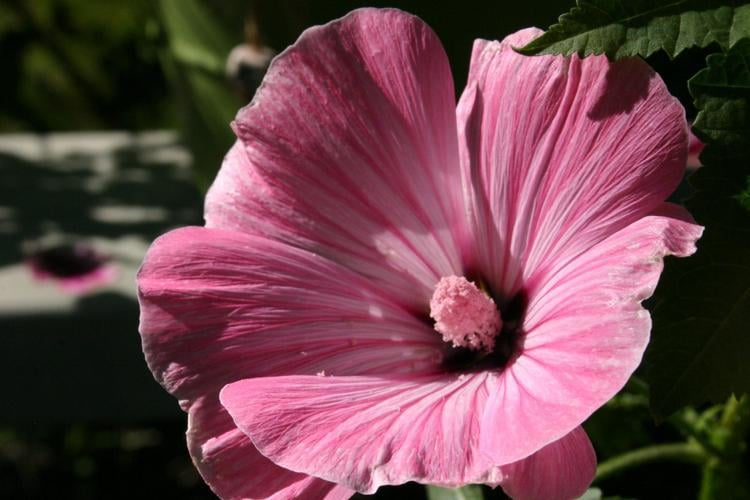
\includegraphics[width=0.14\textwidth,height=0.14\textwidth]{images/input_1.jpg} &
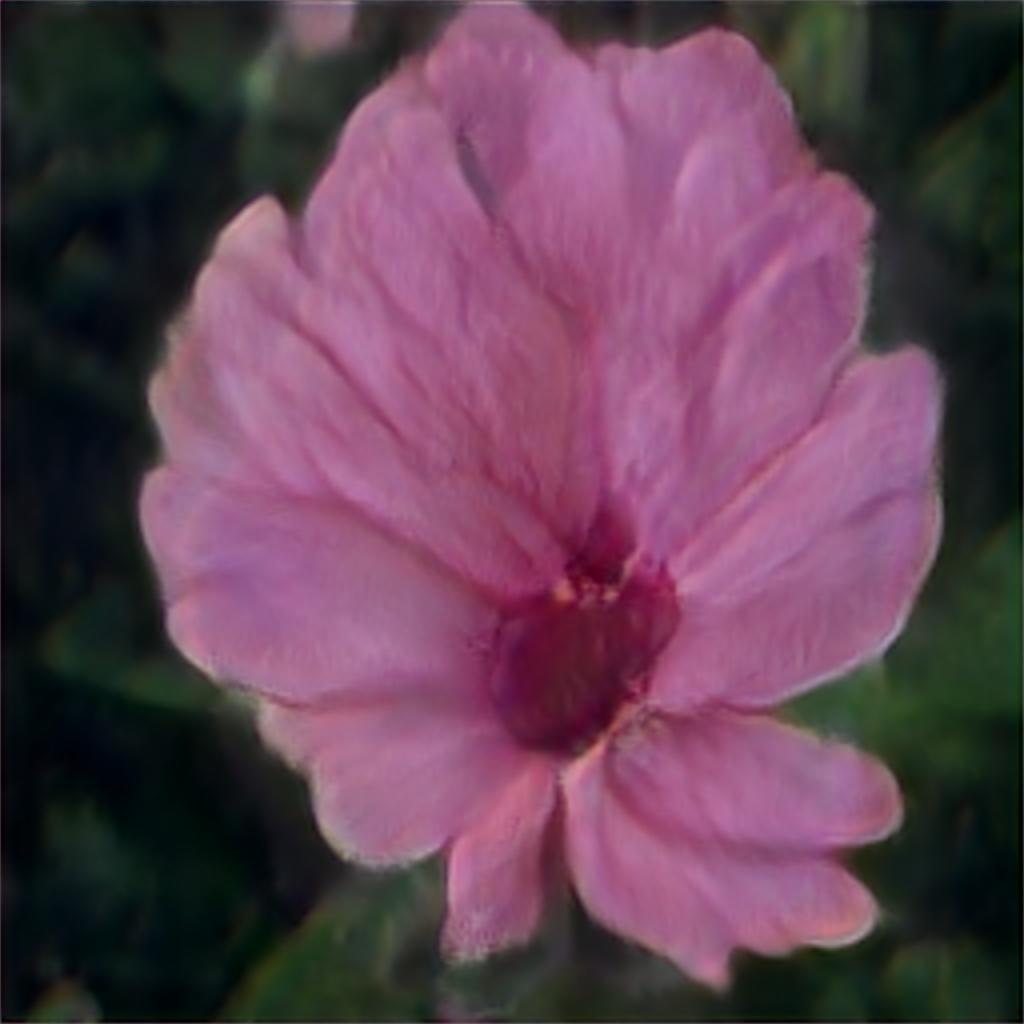
\includegraphics[width=0.14\textwidth,height=0.14\textwidth]{images/1age_output1.jpg} &
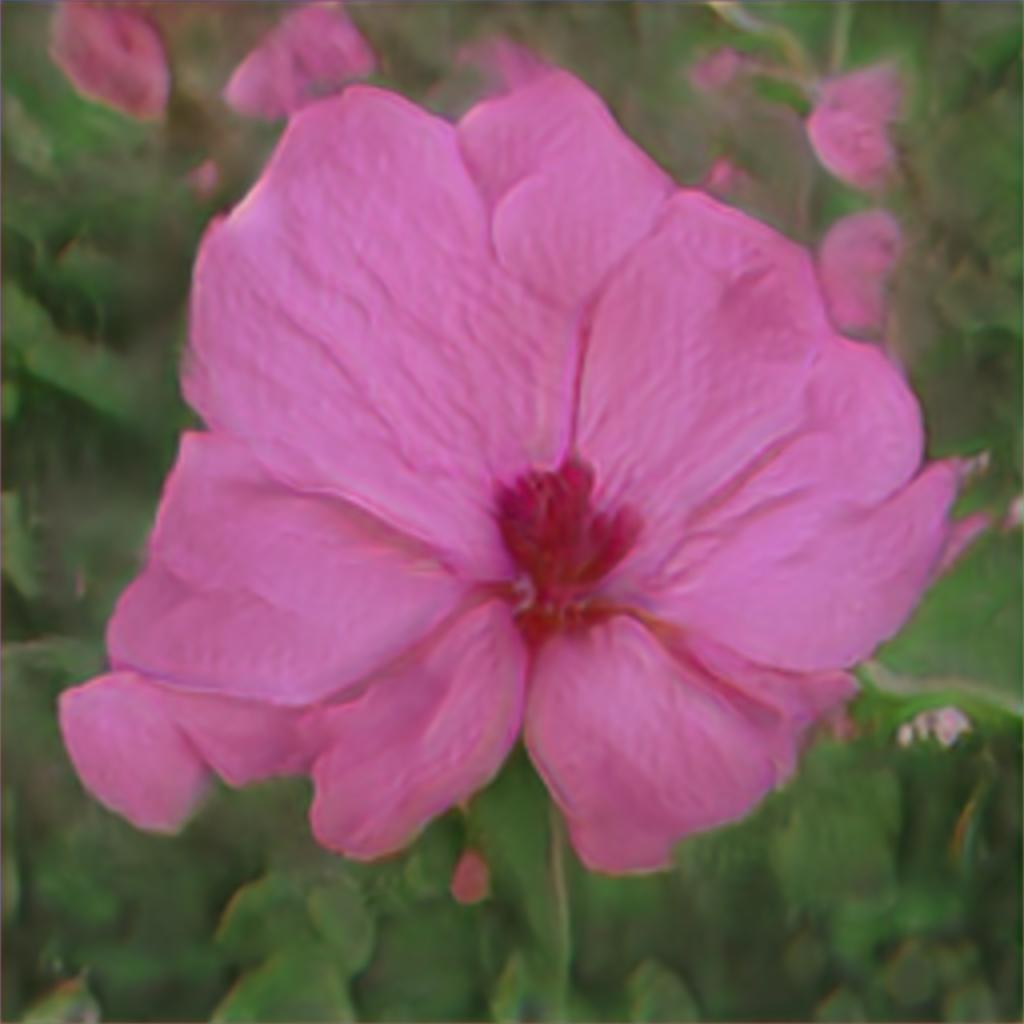
\includegraphics[width=0.14\textwidth,height=0.14\textwidth]{images/1age_output2.jpg} &
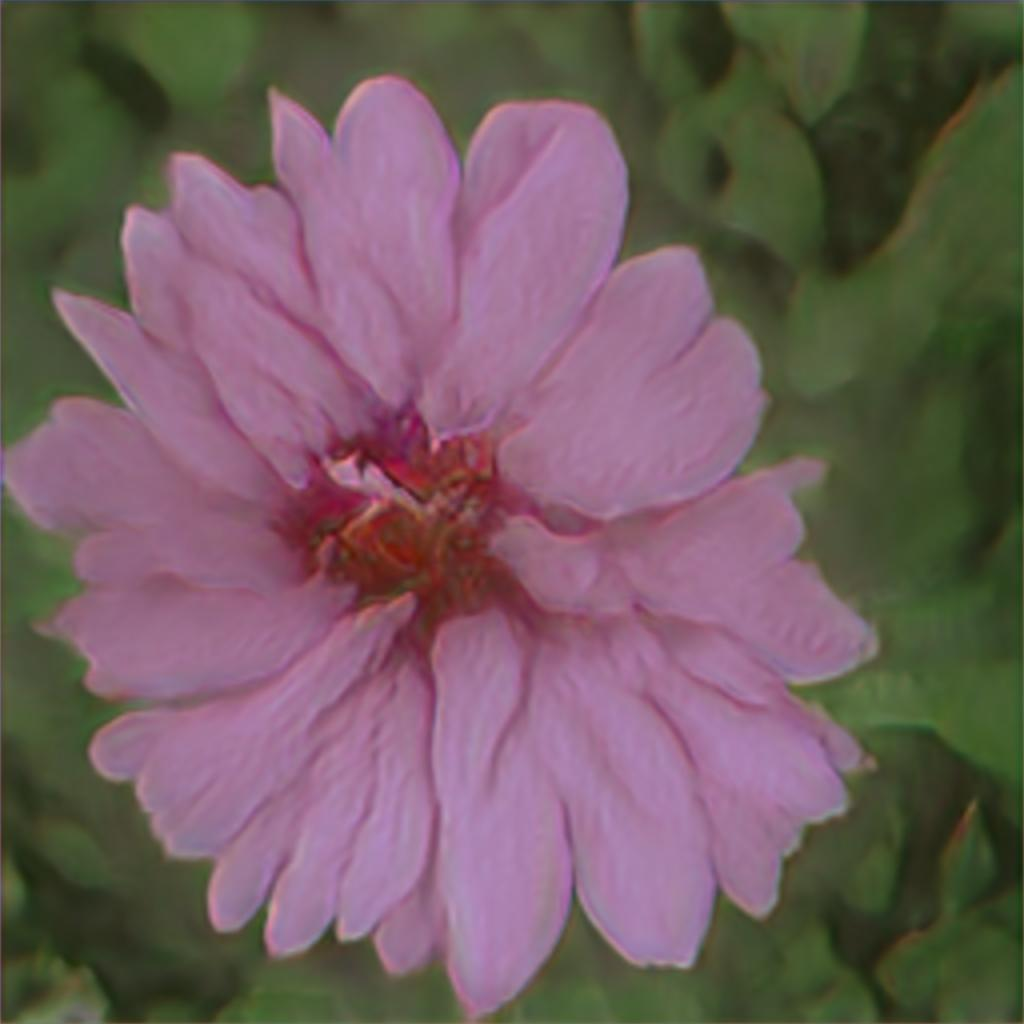
\includegraphics[width=0.14\textwidth,height=0.14\textwidth]{images/1sage_output1.jpg} &
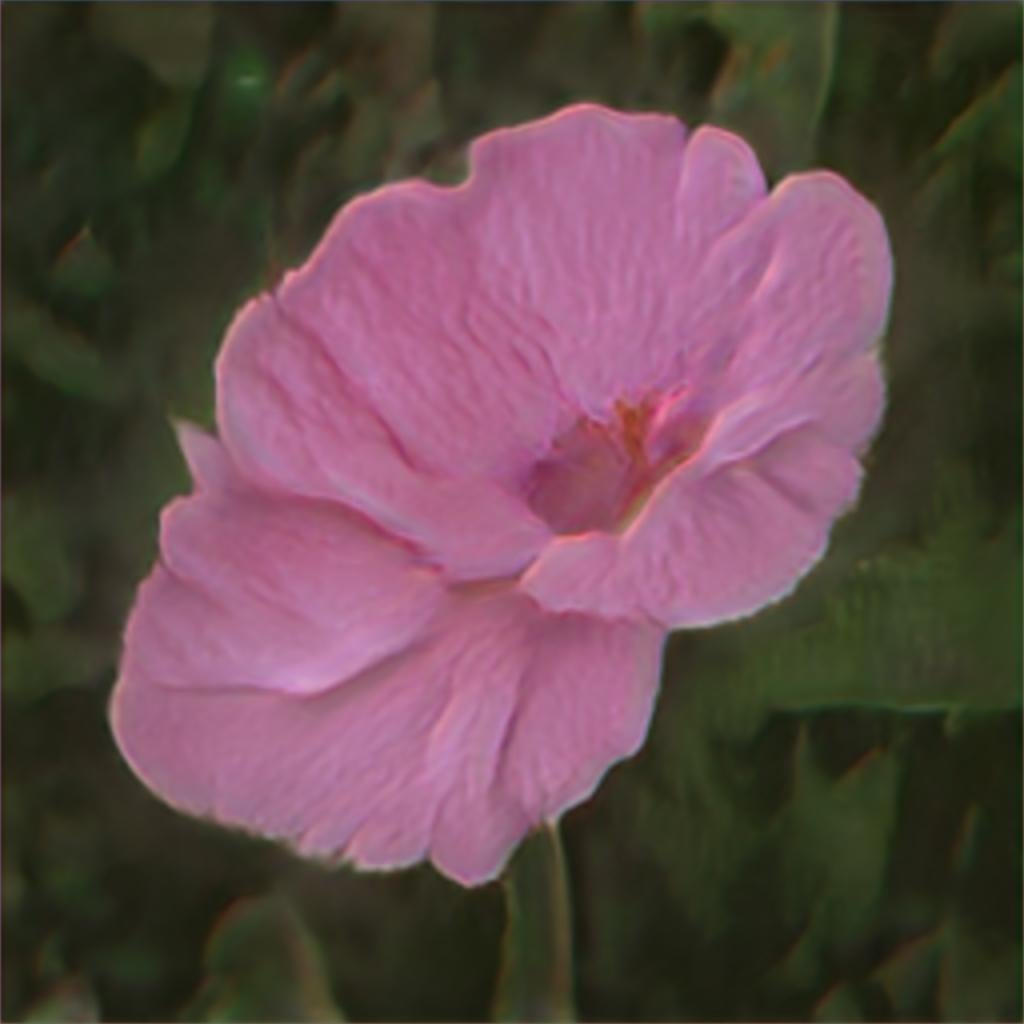
\includegraphics[width=0.14\textwidth,height=0.14\textwidth]{images/1sage_output2.jpg} &
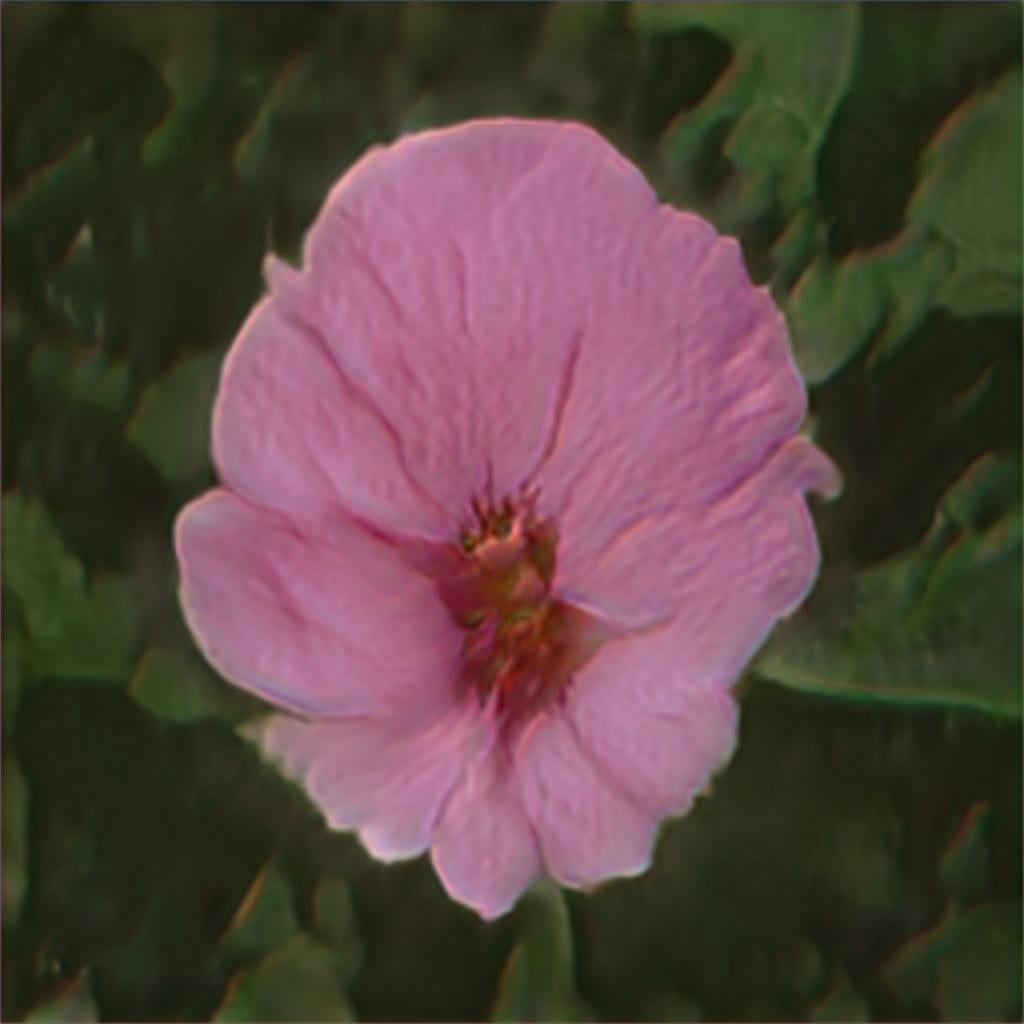
\includegraphics[width=0.14\textwidth,height=0.14\textwidth]{images/1sfsage_output1.jpg} &
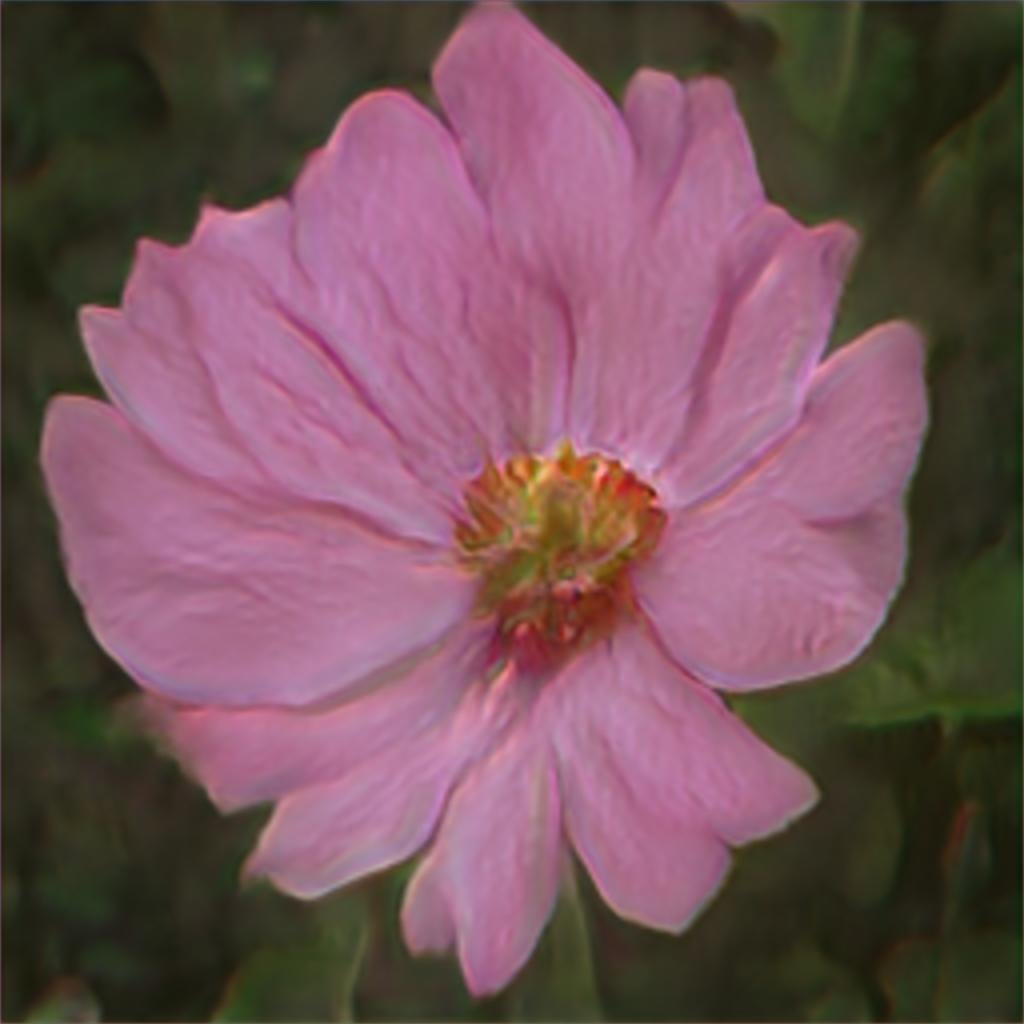
\includegraphics[width=0.14\textwidth,height=0.14\textwidth]{images/1sfsage_output2.jpg}
\\
Input & AGE & AGE & SAGE & SAGE & SFSAGE & SFSAGE
\end{tabular}

\caption{Comparison across AGE, SAGE, and the proposed SFSAGE model under one-shot setting, where a single reference image is used to condition the model during inference.}
\label{fig:qualitative_comparison}
\end{figure}


\begin{figure}[H]
\centering
\setlength{\tabcolsep}{2pt}

\begin{tabular}{ccccccc}
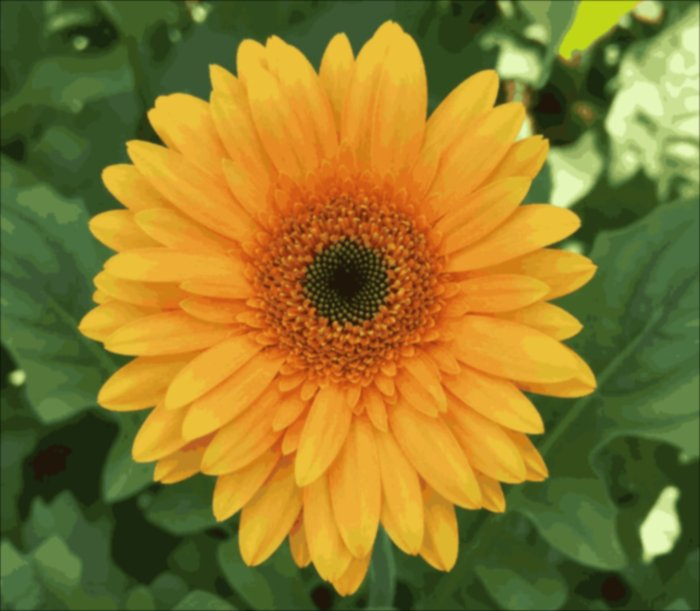
\includegraphics[width=0.14\textwidth,height=0.14\textwidth]{images/input_2.png} &
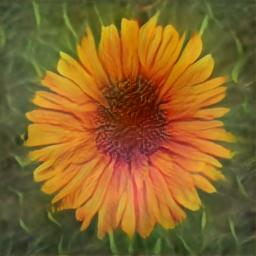
\includegraphics[width=0.14\textwidth,height=0.14\textwidth]{images/2age_output1.jpg} &
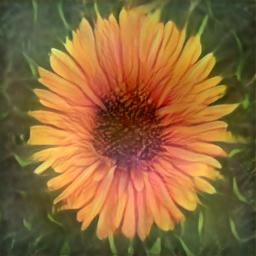
\includegraphics[width=0.14\textwidth,height=0.14\textwidth]{images/2age_output2.jpg} &
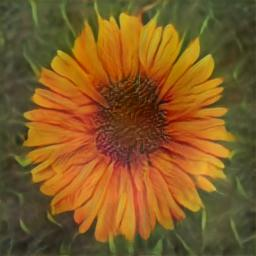
\includegraphics[width=0.14\textwidth,height=0.14\textwidth]{images/2sage_output1.jpg} &
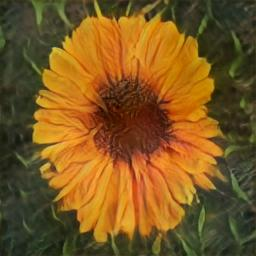
\includegraphics[width=0.14\textwidth,height=0.14\textwidth]{images/2sage_output2.jpg} &
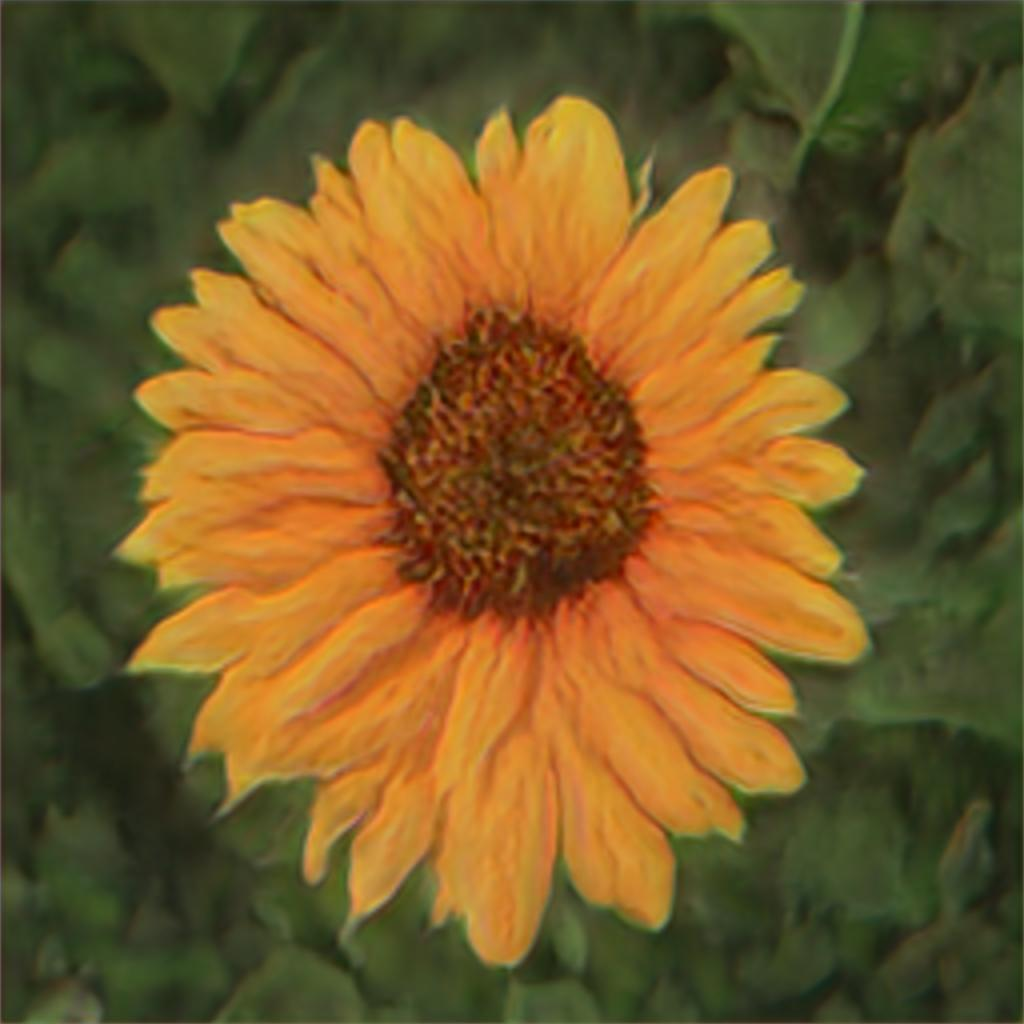
\includegraphics[width=0.14\textwidth,height=0.14\textwidth]{images/2sfsage_output1.jpg} &
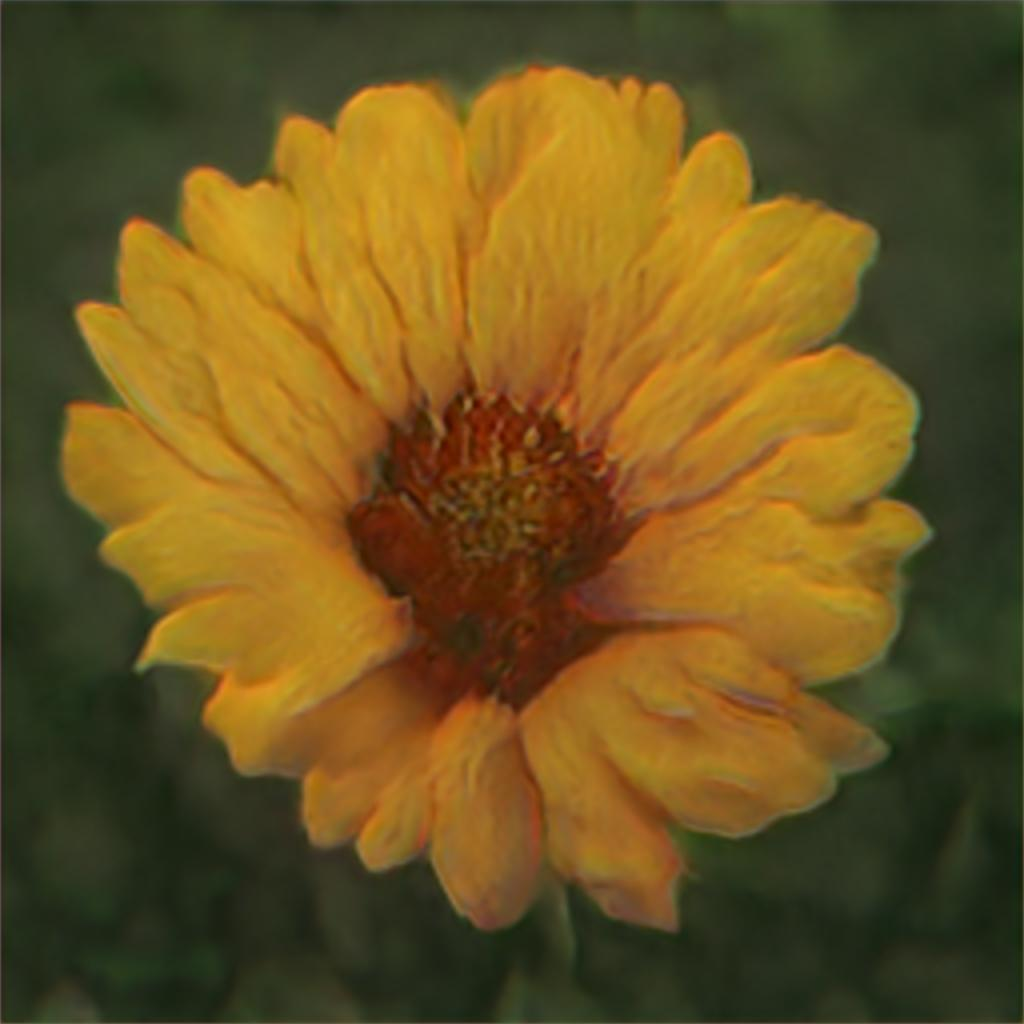
\includegraphics[width=0.14\textwidth,height=0.14\textwidth]{images/2sfsage_ouptut2.jpg}
\\
Input & AGE & AGE & SAGE & SAGE & SFSAGE & SFSAGE
\end{tabular}

\caption{Comparison across AGE, SAGE, and the proposed SFSAGE model under one-shot setting with a different image input.}
\label{fig:qualitative_input2}
\end{figure}

% image names for af:
% input3.png, age_af_output1.jpg, age_af_output2.jpg, sage_af_output1.jpg, sfsage_af_output1.jpg, sage_output2.jpg, sfsage_af_ouptut2.jpg

\begin{figure}[H]
\centering
\setlength{\tabcolsep}{2pt}

\begin{tabular}{ccccccc}
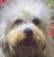
\includegraphics[width=0.14\textwidth,height=0.14\textwidth]{images/input3.jpg} &
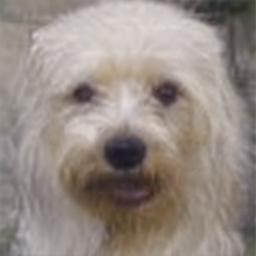
\includegraphics[width=0.14\textwidth,height=0.14\textwidth]{images/age_af_output1.jpg} &
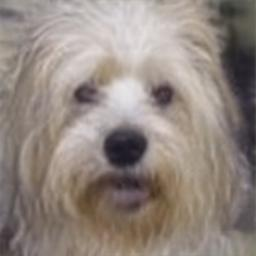
\includegraphics[width=0.14\textwidth,height=0.14\textwidth]{images/age_af_output2.jpg} &
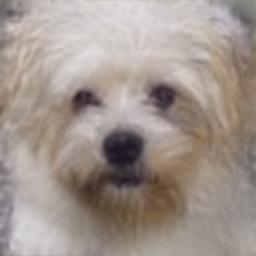
\includegraphics[width=0.14\textwidth,height=0.14\textwidth]{images/sage_af_output1.jpg} &
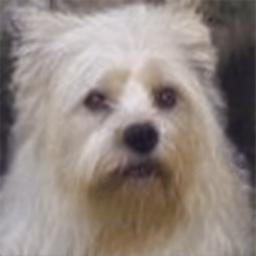
\includegraphics[width=0.14\textwidth,height=0.14\textwidth]{images/sage_output2.jpg} &
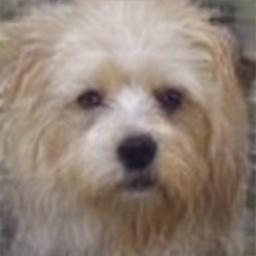
\includegraphics[width=0.14\textwidth,height=0.14\textwidth]{images/sfsage_af_output1.jpg} &
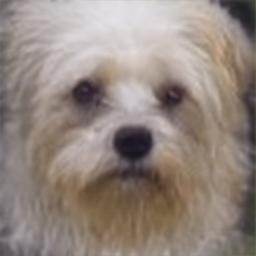
\includegraphics[width=0.14\textwidth,height=0.14\textwidth]{images/sfsage_af_ouptut2.jpg} \\
Input & AGE & AGE & SAGE & SAGE & SFSAGE & SFSAGE
\end{tabular}

\caption{Comparison across AGE, SAGE, and the proposed SFSAGE model on the Animal Faces dataset under one-shot setting. Each model generates two outputs per input image to demonstrate edit diversity and semantic consistency.}
\label{fig:qualitative_animalfaces}
\end{figure}


\subsection{Visual Observations}

\subsubsection{Flowers}

Figures \ref{fig:qualitative_comparison} and \ref{fig:qualitative_input2} describe the qualitative analysis of the results of the edited flowers 
based on the baseline models AGE and SAGE, and the proposed model SFSAGE. The models are compared with regard to their ability to maintain the 
colors properly, the sharpness of the images, the level of contrast, and realism. As shown in Figure \ref{fig:qualitative_comparison}, the proposed 
model performs well in the retention of the pink petal colors from the input images. It also performs much better based on the level of semantic 
consistency. Note that the proposed model also fails to represent the combined red and yellow colors of the pistil from the input images. On the 
other hand, the proposed model performs much better than both the input images in the sharpness of the petal. Although there are inconsistencies 
from the input images, the proposed model also performs much better. In addition, the level of contrast in the proposed model results in the sharpest 
flower among all the models. Further, the advantages of SFSAGE are highlighted by Figure \ref{fig:qualitative_input2}. The sharpness in petal edges 
is better retained by the model compared to AGE and SAGE, which allows for a more photo-realistic and organic rendering. More varied outputs have 
also resulted from SFSAGE; for instance, in one generated image, the flower is presented with a slight tilt, reflecting strong attribute manipulation. 
The model maintains higher clarity, with balanced contrast and natural color distribution, while AGE slightly looks pale with reduced contrast in 
areas, which is somewhat settled by SAGE as it balances the contrast. Overall, the 65 generated flower images produced by SFSAGE are the sharpest, 
most realistic, and visually consistent as compared to the other models being tested.

\subsubsection{Animal Faces}

Figure \ref{fig:qualitative_animalfaces} provides a comparison of the outputs produced by the AGE, SAGE, and proposed SFSAGE model on the 
Animal Faces data set using a picture of a dog as input. As observed, the outputs produced by the models have managed to maintain the color 
and texture of the input data, implying success by these models in maintaining basic characteristics produced by each model. Considering the 
clarity and image properties, all the outputs produced by these models can be considered similar, since there is minimal blurring effect and 
texture preservation on the fur of the input image. Consistency and overall properties, on the other hand, differ significantly, since there 
is more diversity apparent in the outputs produced by the AGE and SAGE models, with a slight difference in orientation between the two outcomes 
produced by each model. The more consistent results produced by the proposed SFSAGE model, on the contrary, demonstrate success towards 
maintaining integrity while providing semantic edits. Also, there are some minor enhancements in the realism of the output, whereby the output 
from SFSAGE shows slightly more coherent shading and blending of the fur patterns. This indicates that although all these models demonstrate 
the ability to sustain basic attributes like color and texture, the SFSAGE model has the best consistency in output.

\section{Failure Cases and Limitations}

During experimentation and evaluation of the FeatureSAGE framework, two main limitations were observed:

\begin{enumerate}
    \item \textbf{Dependence on a pretrained StyleGAN2 generator.} FeatureSAGE inherits the coverage and biases of the pretrained StyleGAN2 generator. If the generator does not adequately represent certain categories or visual attributes, those gaps may appear in the generated outputs. This constraint limits the framework to domains where an appropriate pretrained StyleGAN2 model is available and sufficiently aligned with the target data.

    \item \textbf{Computational overhead.} Integrating the StyleFeatureEditor inverter and Feature Editor increases the computational cost relative to the baseline SAGE setup. These components improve reconstruction and feature-level editing, but they require additional generator passes and feature-tensor operations. As a result, the framework requires more GPU memory and can slow inference or training, especially when scaling to larger datasets or time-sensitive applications.
\end{enumerate}

These limitations indicate that the reported quality improvements involve a trade-off between image fidelity and computational efficiency. They also motivate future work on lighter inversion modules, more efficient feature editing, and evaluation with generator backbones beyond StyleGAN2.

\chapter{Summary, Conclusion and Recommendation}

\section{Summary of Findings}

\subsection{Summary of Contributions}

\paragraph{1. Integration of StyleFeatureEditor (SFE) Encoder} 
FeatureSAGE integrates StyleFeatureEditor Encoder on the original SAGE framework, enabling improved latent representations that better 
capture distributional characteristics of the data across resolutions.

\paragraph{2. Integration of Feature Editor} 
The Feature Editor module allows fine-grained and semantically consistent modifications by operating directly on intermediate feature representations, enhancing the 
expressiveness of attribute edits.

\paragraph{3. Resolution-Dependent and Dataset-Adaptive Editing} 
FeatureSAGE adapts its editing strategies according to both image resolution and dataset characteristics, ensuring appropriate trade-offs between edit diversity, 
stability, and realism.

\paragraph{4. Comprehensive Benchmarking Against Baselines} 
The framework demonstrates robust performance across structurally diverse datasets (Flowers and Animal Faces) and multiple resolutions, providing a generalizable 
approach to few-shot image generation while balancing perceptual expressiveness and identity preservation.

\subsection{Empirical Outcomes}

\paragraph{Quantitative Performance} 
FeatureSAGE consistently improves distributional realism across datasets and resolutions. Key metrics include:

\begin{itemize}
    \item \textbf{FID improvements:} At $1024 \times 1024$, FeatureSAGE reduces FID by 25.9\% on Flowers (45.60 vs. 61.57 for AGE) and 15.8\% (vs. 54.17 for SAGE), and by 20.2\% on Animal Faces (49.60 vs. 62.13 for AGE) and 18.6\% (vs. 60.92 for SAGE). At $256 \times 256$ on Flowers, reductions are 15.0\% (vs. AGE) and 9.1\% (vs. SAGE).
    \item \textbf{LPIPS performance:} On Flowers at $1024 \times 1024$, FeatureSAGE achieves an LPIPS of 0.4209, which is 7.0\% lower than SAGE (0.4528) and 2.5\% higher than AGE (0.4108), maintaining competitive perceptual diversity. At $256 \times 256$, LPIPS decreases to 0.1309, representing a 37.2\% reduction compared to SAGE (0.2085) and 37.9\% compared to AGE (0.2108). On Animal Faces at $1024 \times 1024$, LPIPS is 0.4811, within 1.2\% of SAGE (0.4867) and 4.4\% of AGE (0.5033).
\end{itemize}

\paragraph{Dataset and Resolution-Adaptive Trends} 
The framework demonstrates resolution-dependent behavior: 
\begin{itemize}
    \item At $1024 \times 1024$ resolution, FeatureSAGE achieves substantial FID improvements (15.8-25.9\%) while maintaining LPIPS within 7.0\% of baseline methods across both datasets.
    \item At $256 \times 256$ resolution on Flowers, FID improvements are smaller (9.1-15.0\%) but accompanied by larger LPIPS reductions (37.2-37.9\%), indicating reduced perceptual diversity at lower resolutions.
    \item LPIPS values decrease substantially from high to low resolution on Flowers (0.4209 to 0.1309), while the pattern differs across datasets based on their structural characteristics.
\end{itemize}

\subsection{Limitations}

Though FeatureSAGE holds promise in attribute group editing and limited example image synthesis, some constraints observed during testing indicate that there is scope for further research. The first is the reliance on a pre-trained StyleGAN2 generator, which restricts the application of this tool only to domains where such generators have been developed, and any biases in the model may have been passed on to the output. The second is the potential performance impact of integrating the StyleFeatureEditor with the Feature Editor, which increases computational requirements. Future research could focus on other base models, incorporate a multi-level feature approach to improve consistency between edits, optimize computation for more general or faster models, and extend few-shot adaptation to work well even on entirely new classes.

\section{Future Work}

Future research may focus on reducing the computational overhead introduced by the StyleFeatureEditor inverter and Feature Editor. More efficient inversion or feature-editing modules could preserve the FID improvements reported in this study while lowering GPU memory use and inference time.

Another direction is to evaluate FeatureSAGE with generator backbones beyond StyleGAN2. Since the present study is limited to the StyleGAN2-based SAGE pipeline, testing other generator architectures would clarify whether the same feature-level editing strategy generalizes beyond the current framework.

Future work may also examine multi-level feature editing. The current implementation uses an intermediate feature tensor for feature injection; extending the approach to multiple feature levels could further test whether local detail preservation and semantic consistency can be improved without sacrificing perceptual variation.


\subsection{Conclusion}

% Restate the problem and proposed solution.

% Summarize how FeatureSAGE addresses the limitations of SAGE.

% Final remarks on the impact for few-shot image generation and editing.




\begin{doublespacing}
\clearpage
\renewcommand{\bibname}{REFERENCES}
\addcontentsline{toc}{chapter}{REFERENCES}
\bibliographystyle{apacite}
\bibliography{references}
\end{doublespacing}


\clearpage
\vspace*{-1cm}
{\centering\normalfont\bfseries\fontsize{14}{16}\selectfont APPENDICES\par}
\addcontentsline{toc}{chapter}{APPENDICES}
\vspace{36pt}

% ===============
\section*{Appendix A. Overall Similarity Result}
\addcontentsline{toc}{section}{Appendix A. Overall Similarity Result}
\begin{figure}[H]
	\centering
	\fbox{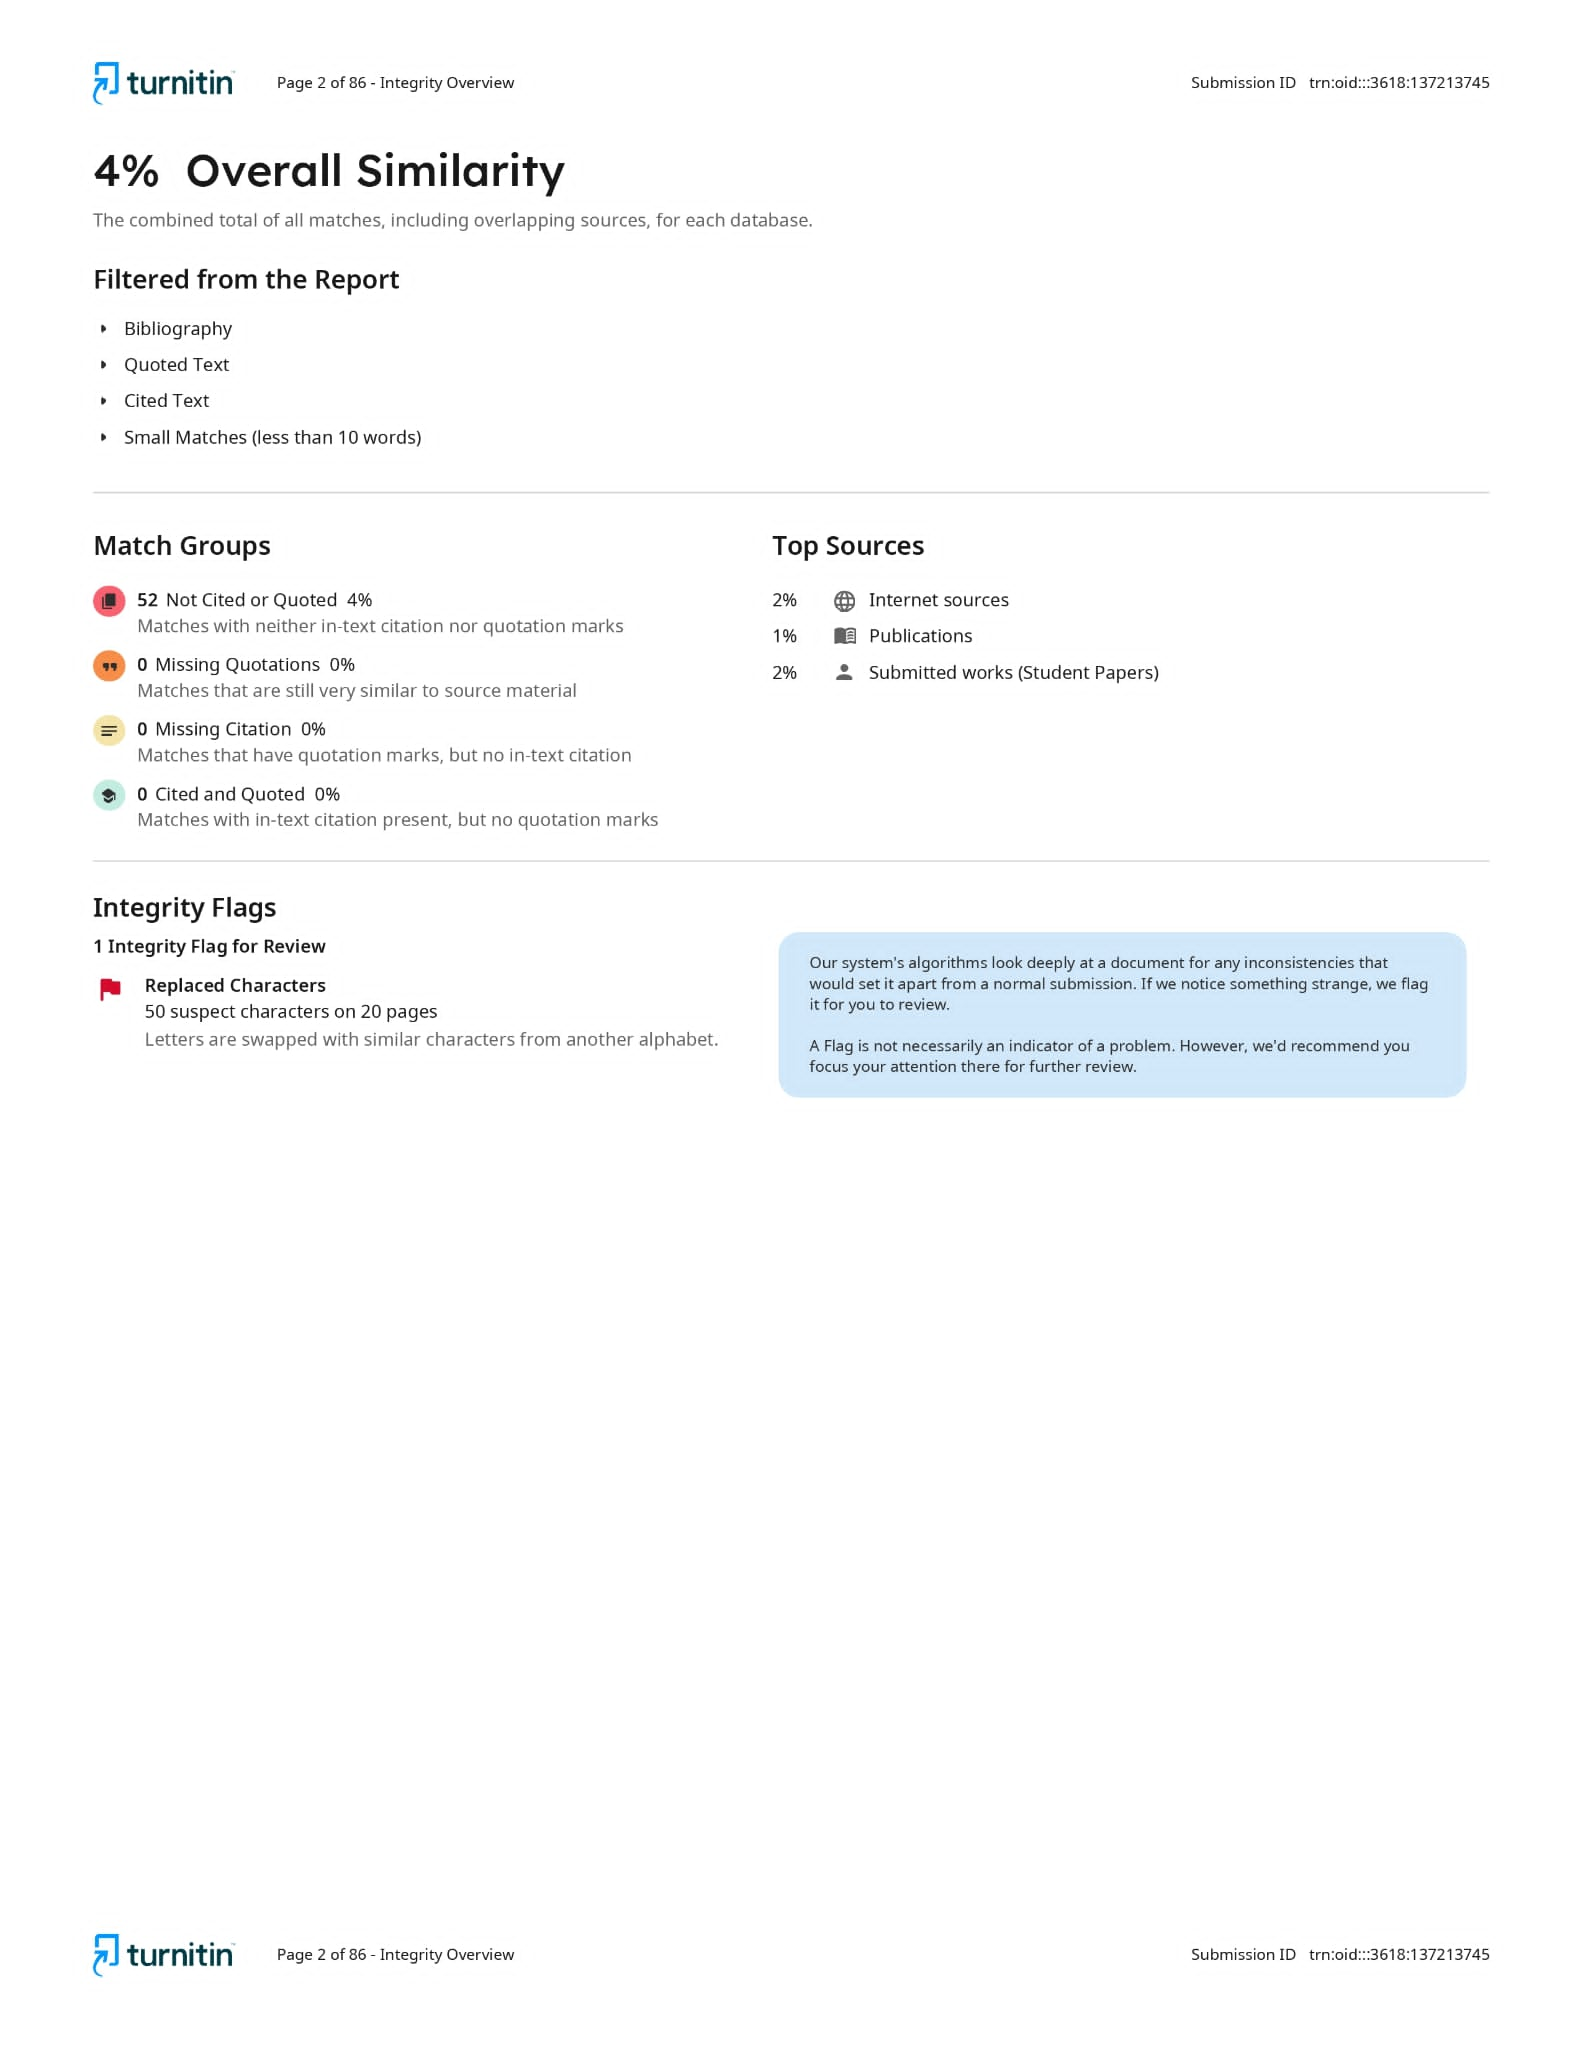
\includegraphics[
		width=\dimexpr\textwidth-2\fboxrule,
		height=0.75\textheight,
		keepaspectratio=true
		]{images/turnitin2.png}}
\end{figure}

% ===============
\clearpage
\section*{Appendix B. AI Detection Result}
\addcontentsline{toc}{section}{Appendix B. AI Detection Result}
\begin{figure}[H]
	\centering
	\fbox{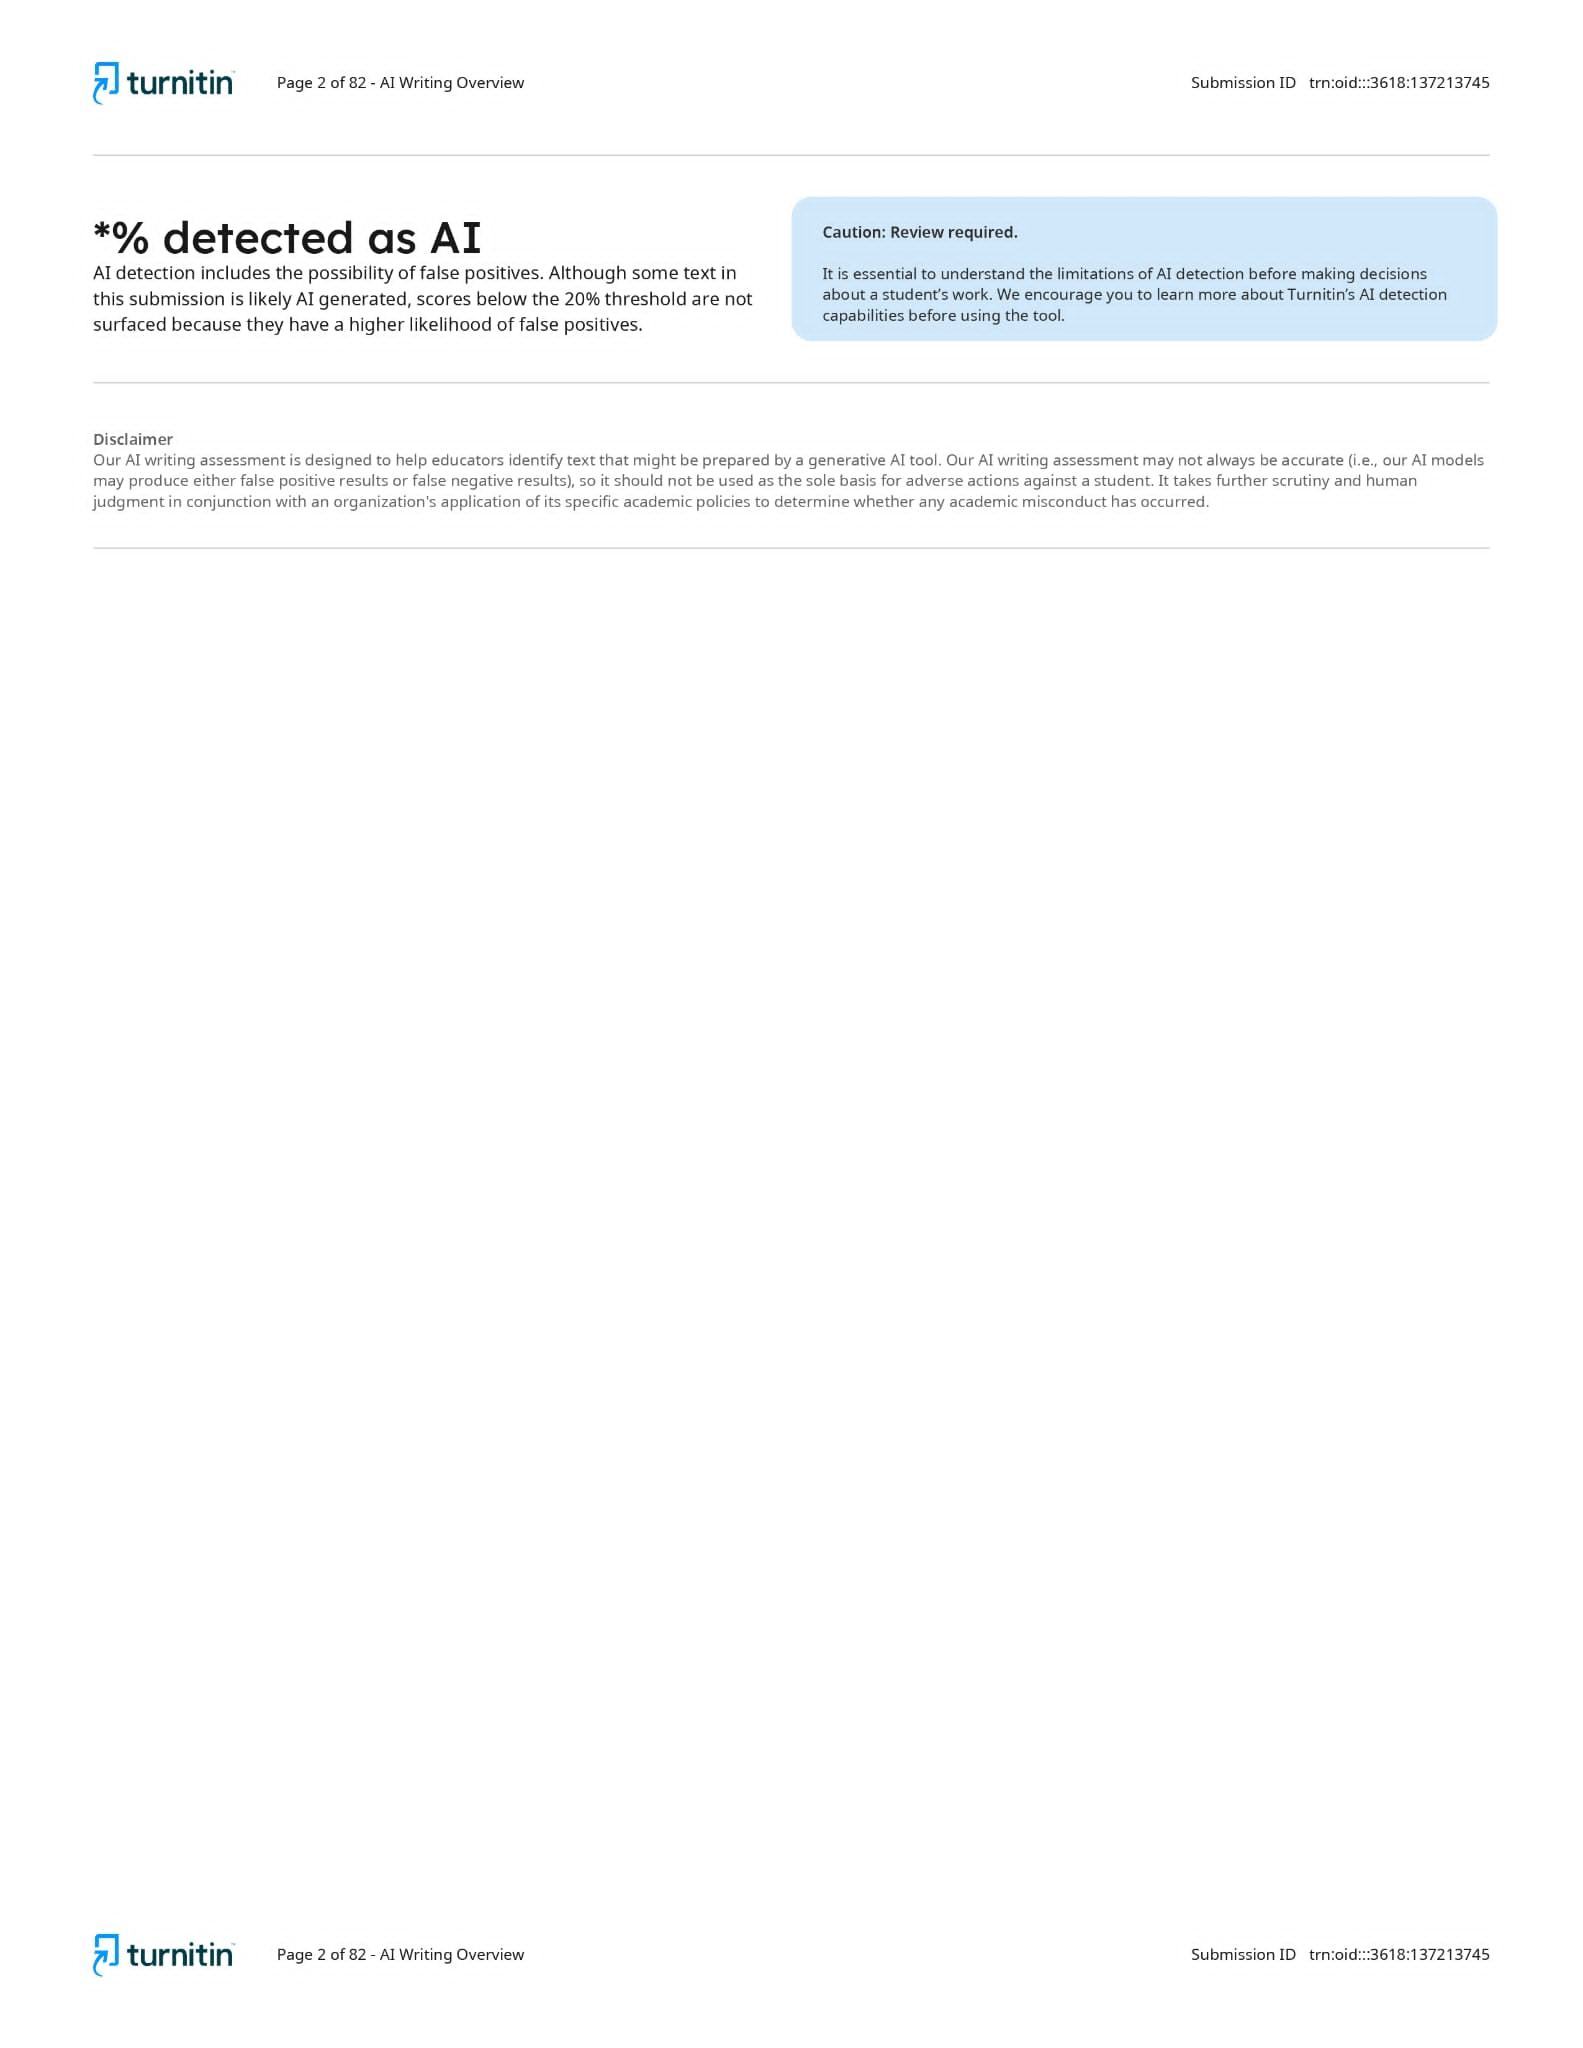
\includegraphics[
		width=\dimexpr\textwidth-2\fboxrule,
		height=0.85\textheight,
		keepaspectratio=true
		]{images/turnitin.png}}
\end{figure}

% ===============
\clearpage
\section*{Appendix C. Deed of Assignment}
\addcontentsline{toc}{section}{Appendix C. Deed of Assignment}
\begin{figure}[H]
	\centering
	\fbox{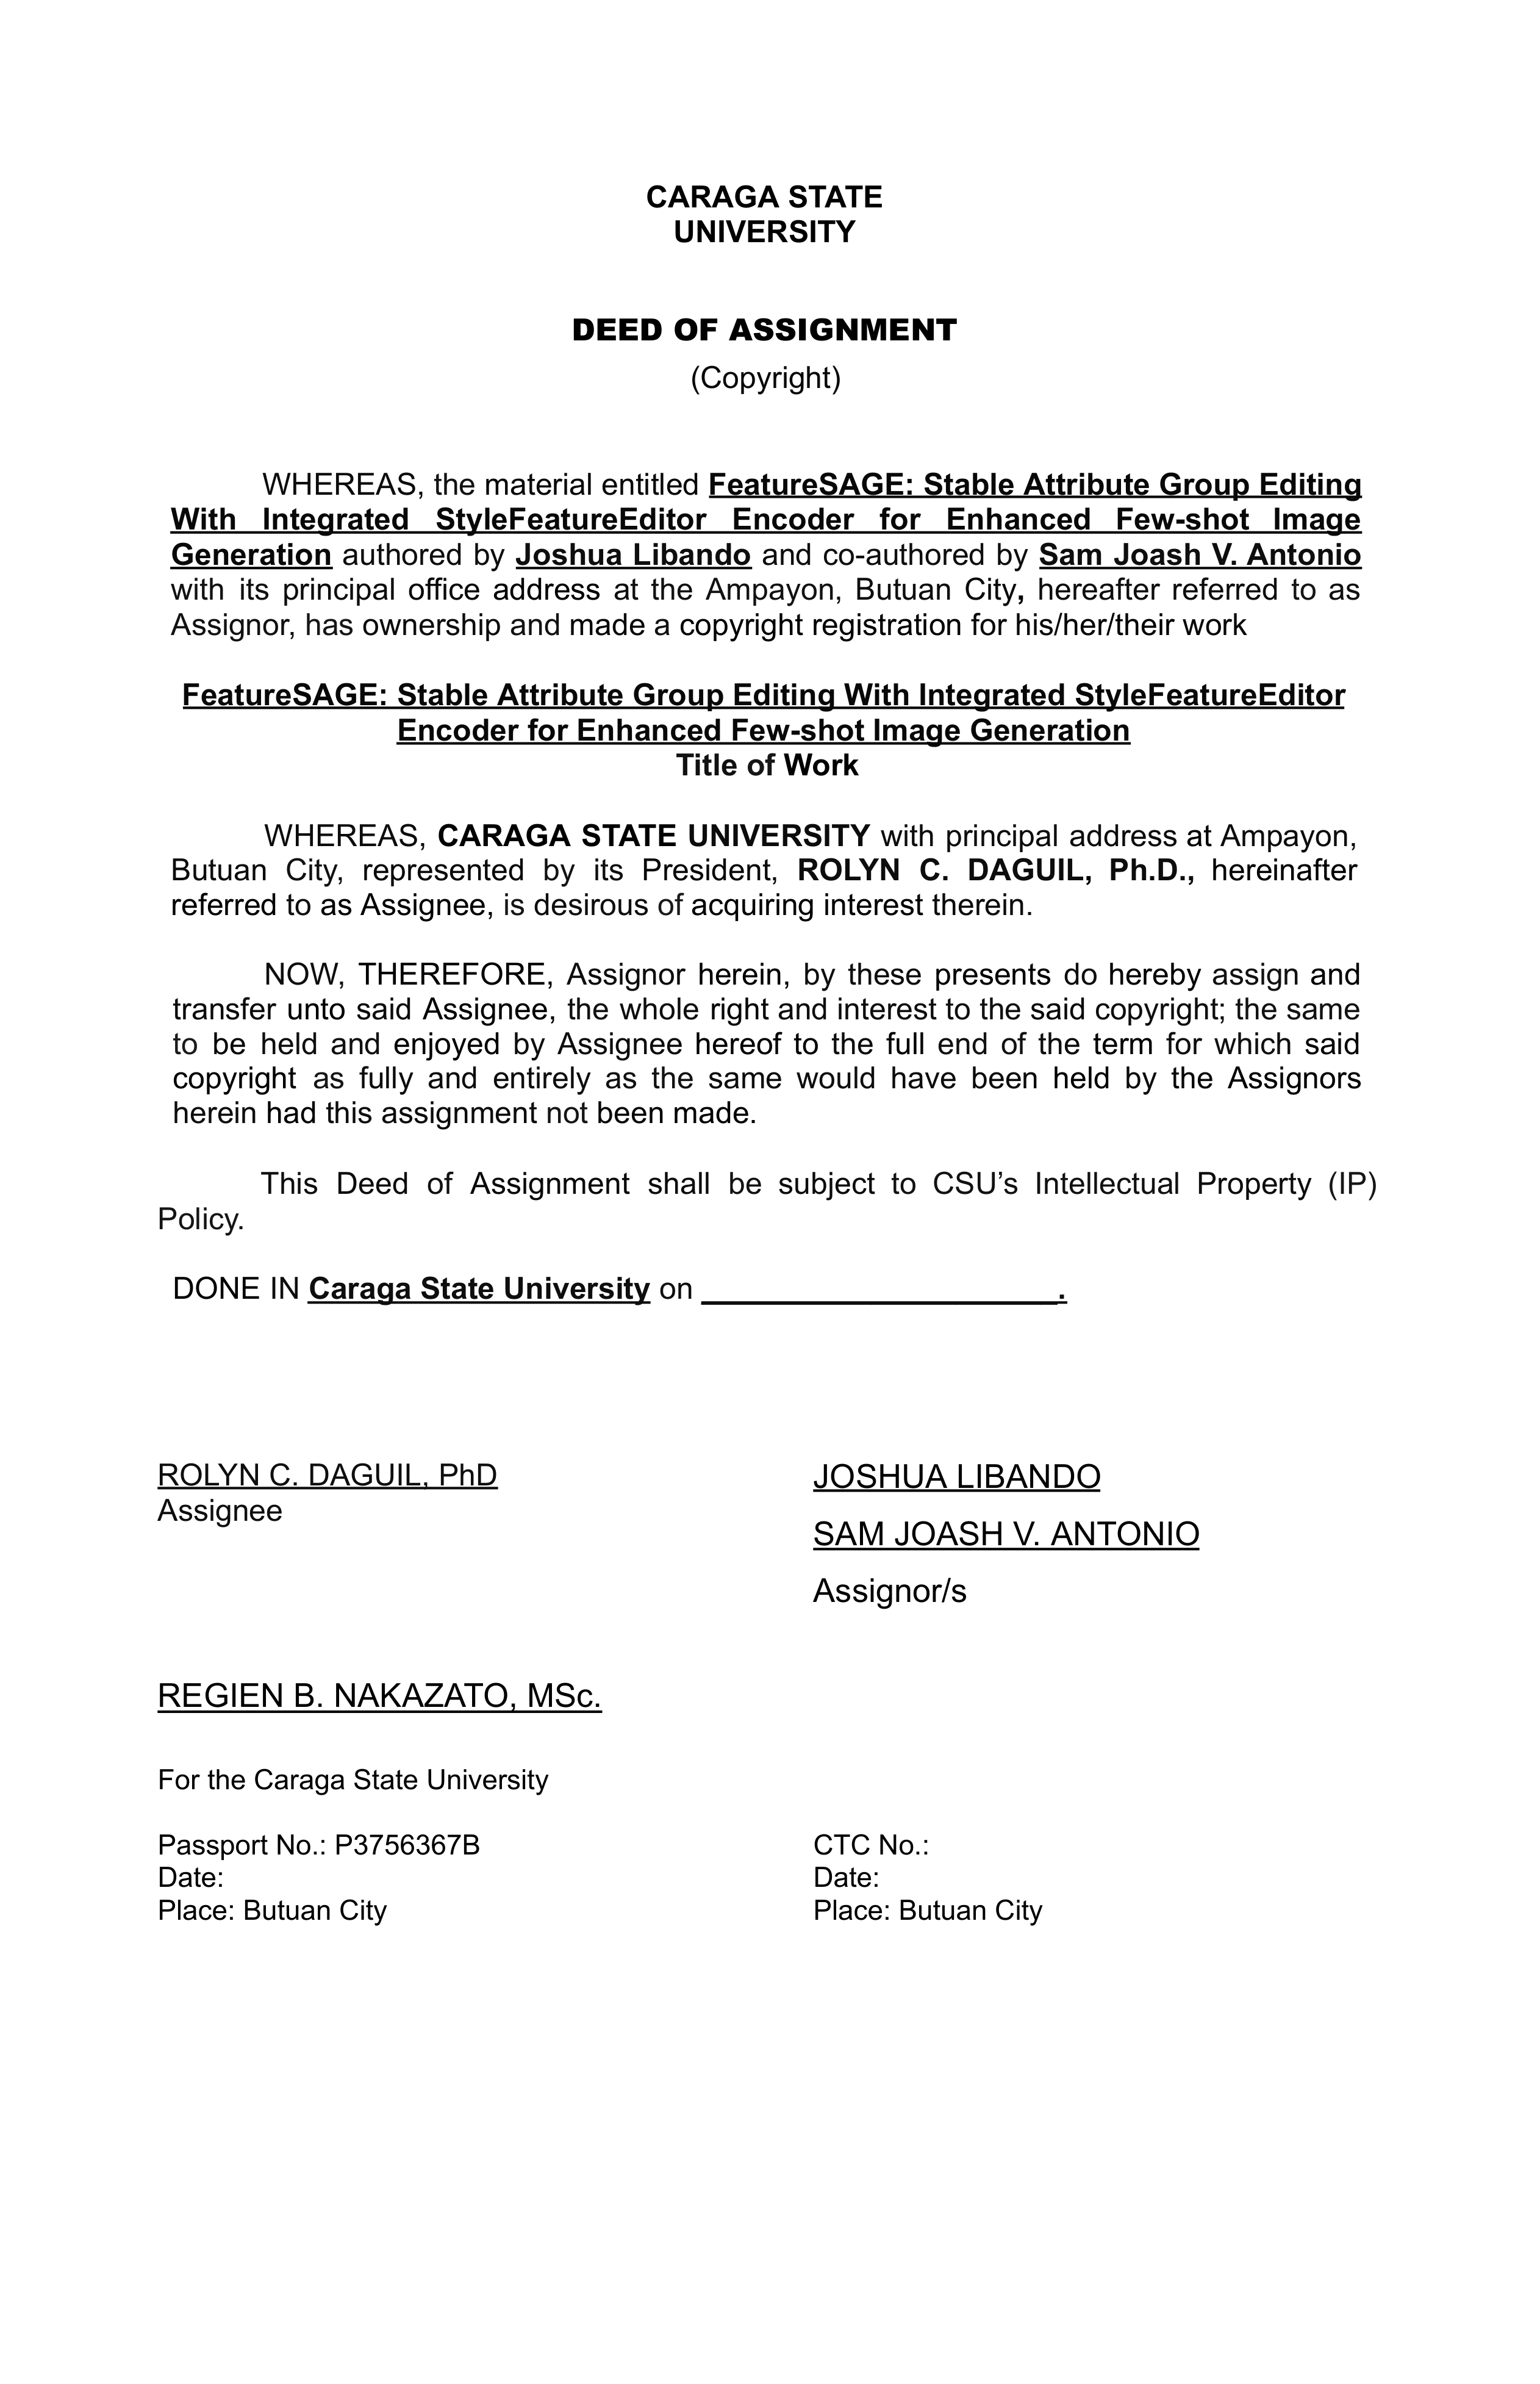
\includegraphics[
		width=\dimexpr\textwidth-2\fboxrule,
		height=0.92\textheight,
		keepaspectratio=true
		]{images/ip1}}
\end{figure}
\begin{figure}[H]
	\centering
	\fbox{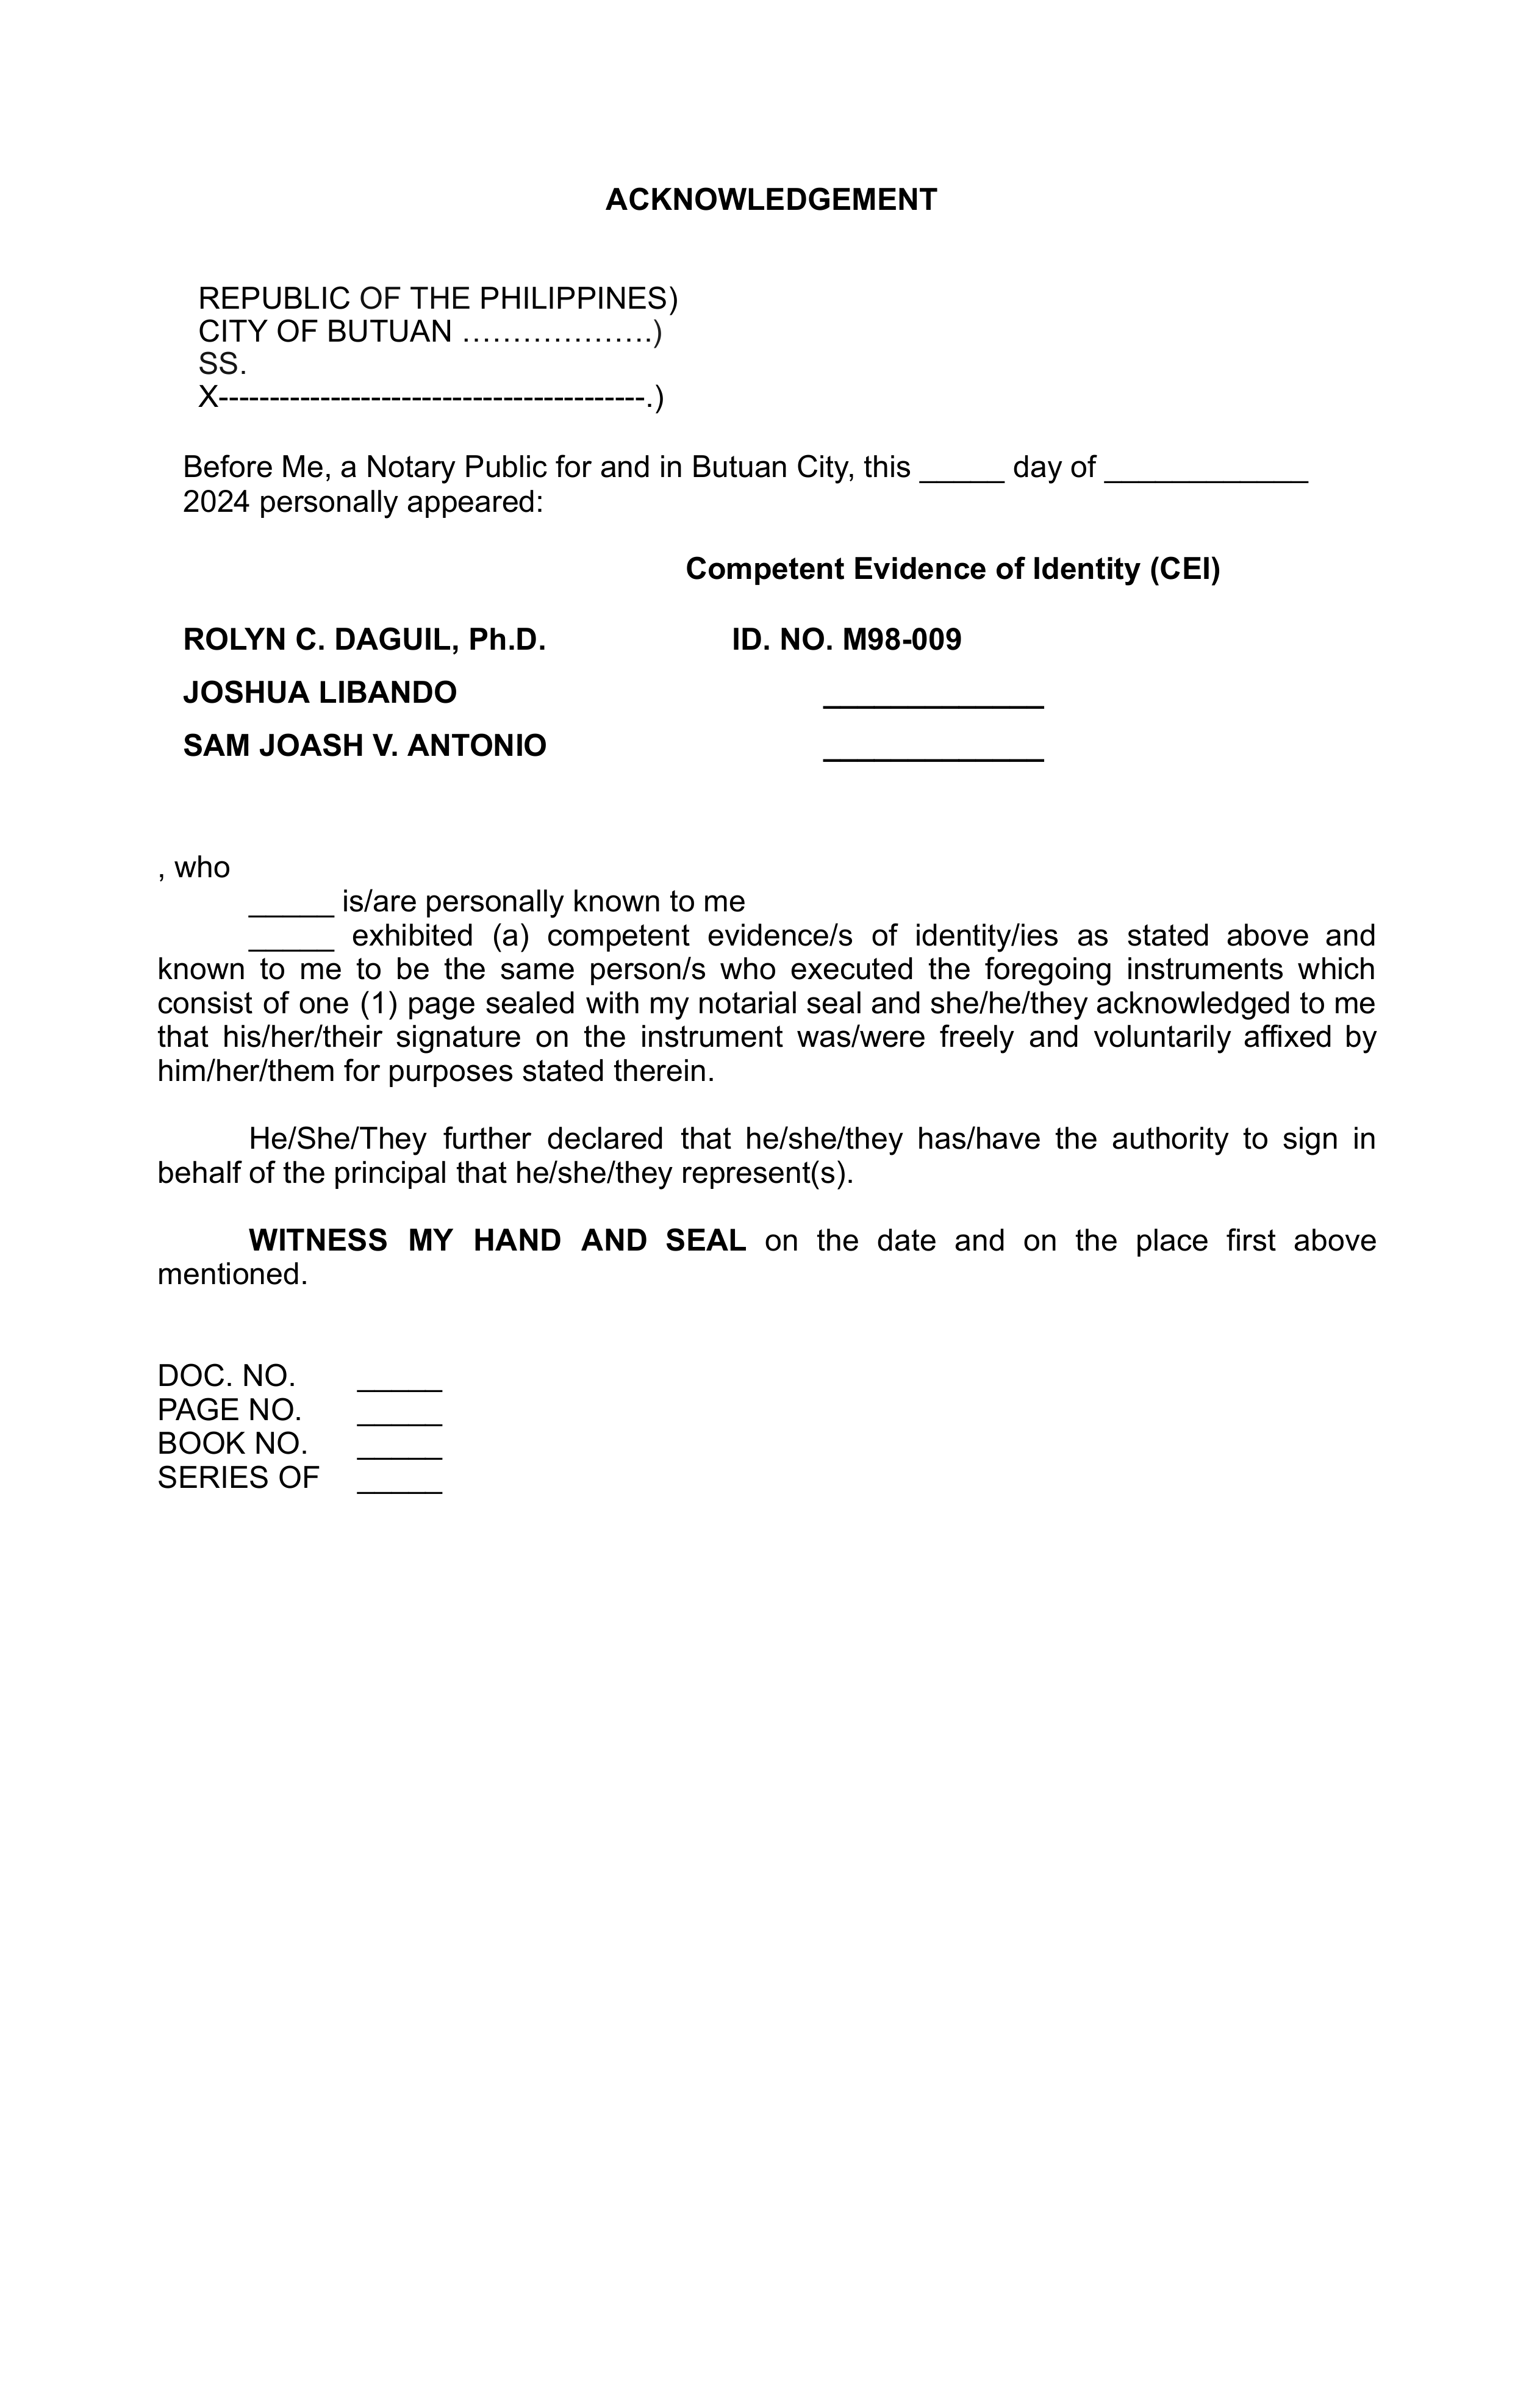
\includegraphics[
		width=\dimexpr\textwidth-2\fboxrule,
		height=0.85\textheight,
		keepaspectratio=true
		]{images/ip2}}
\end{figure}
\clearpage

% ===============
\clearpage
\section*{Appendix D. Certification of Substantial Use of University Resources}
\addcontentsline{toc}{section}{Appendix D. Certification of Substantial Use of University Resources}
\begin{figure}[H]
	\centering
	\fbox{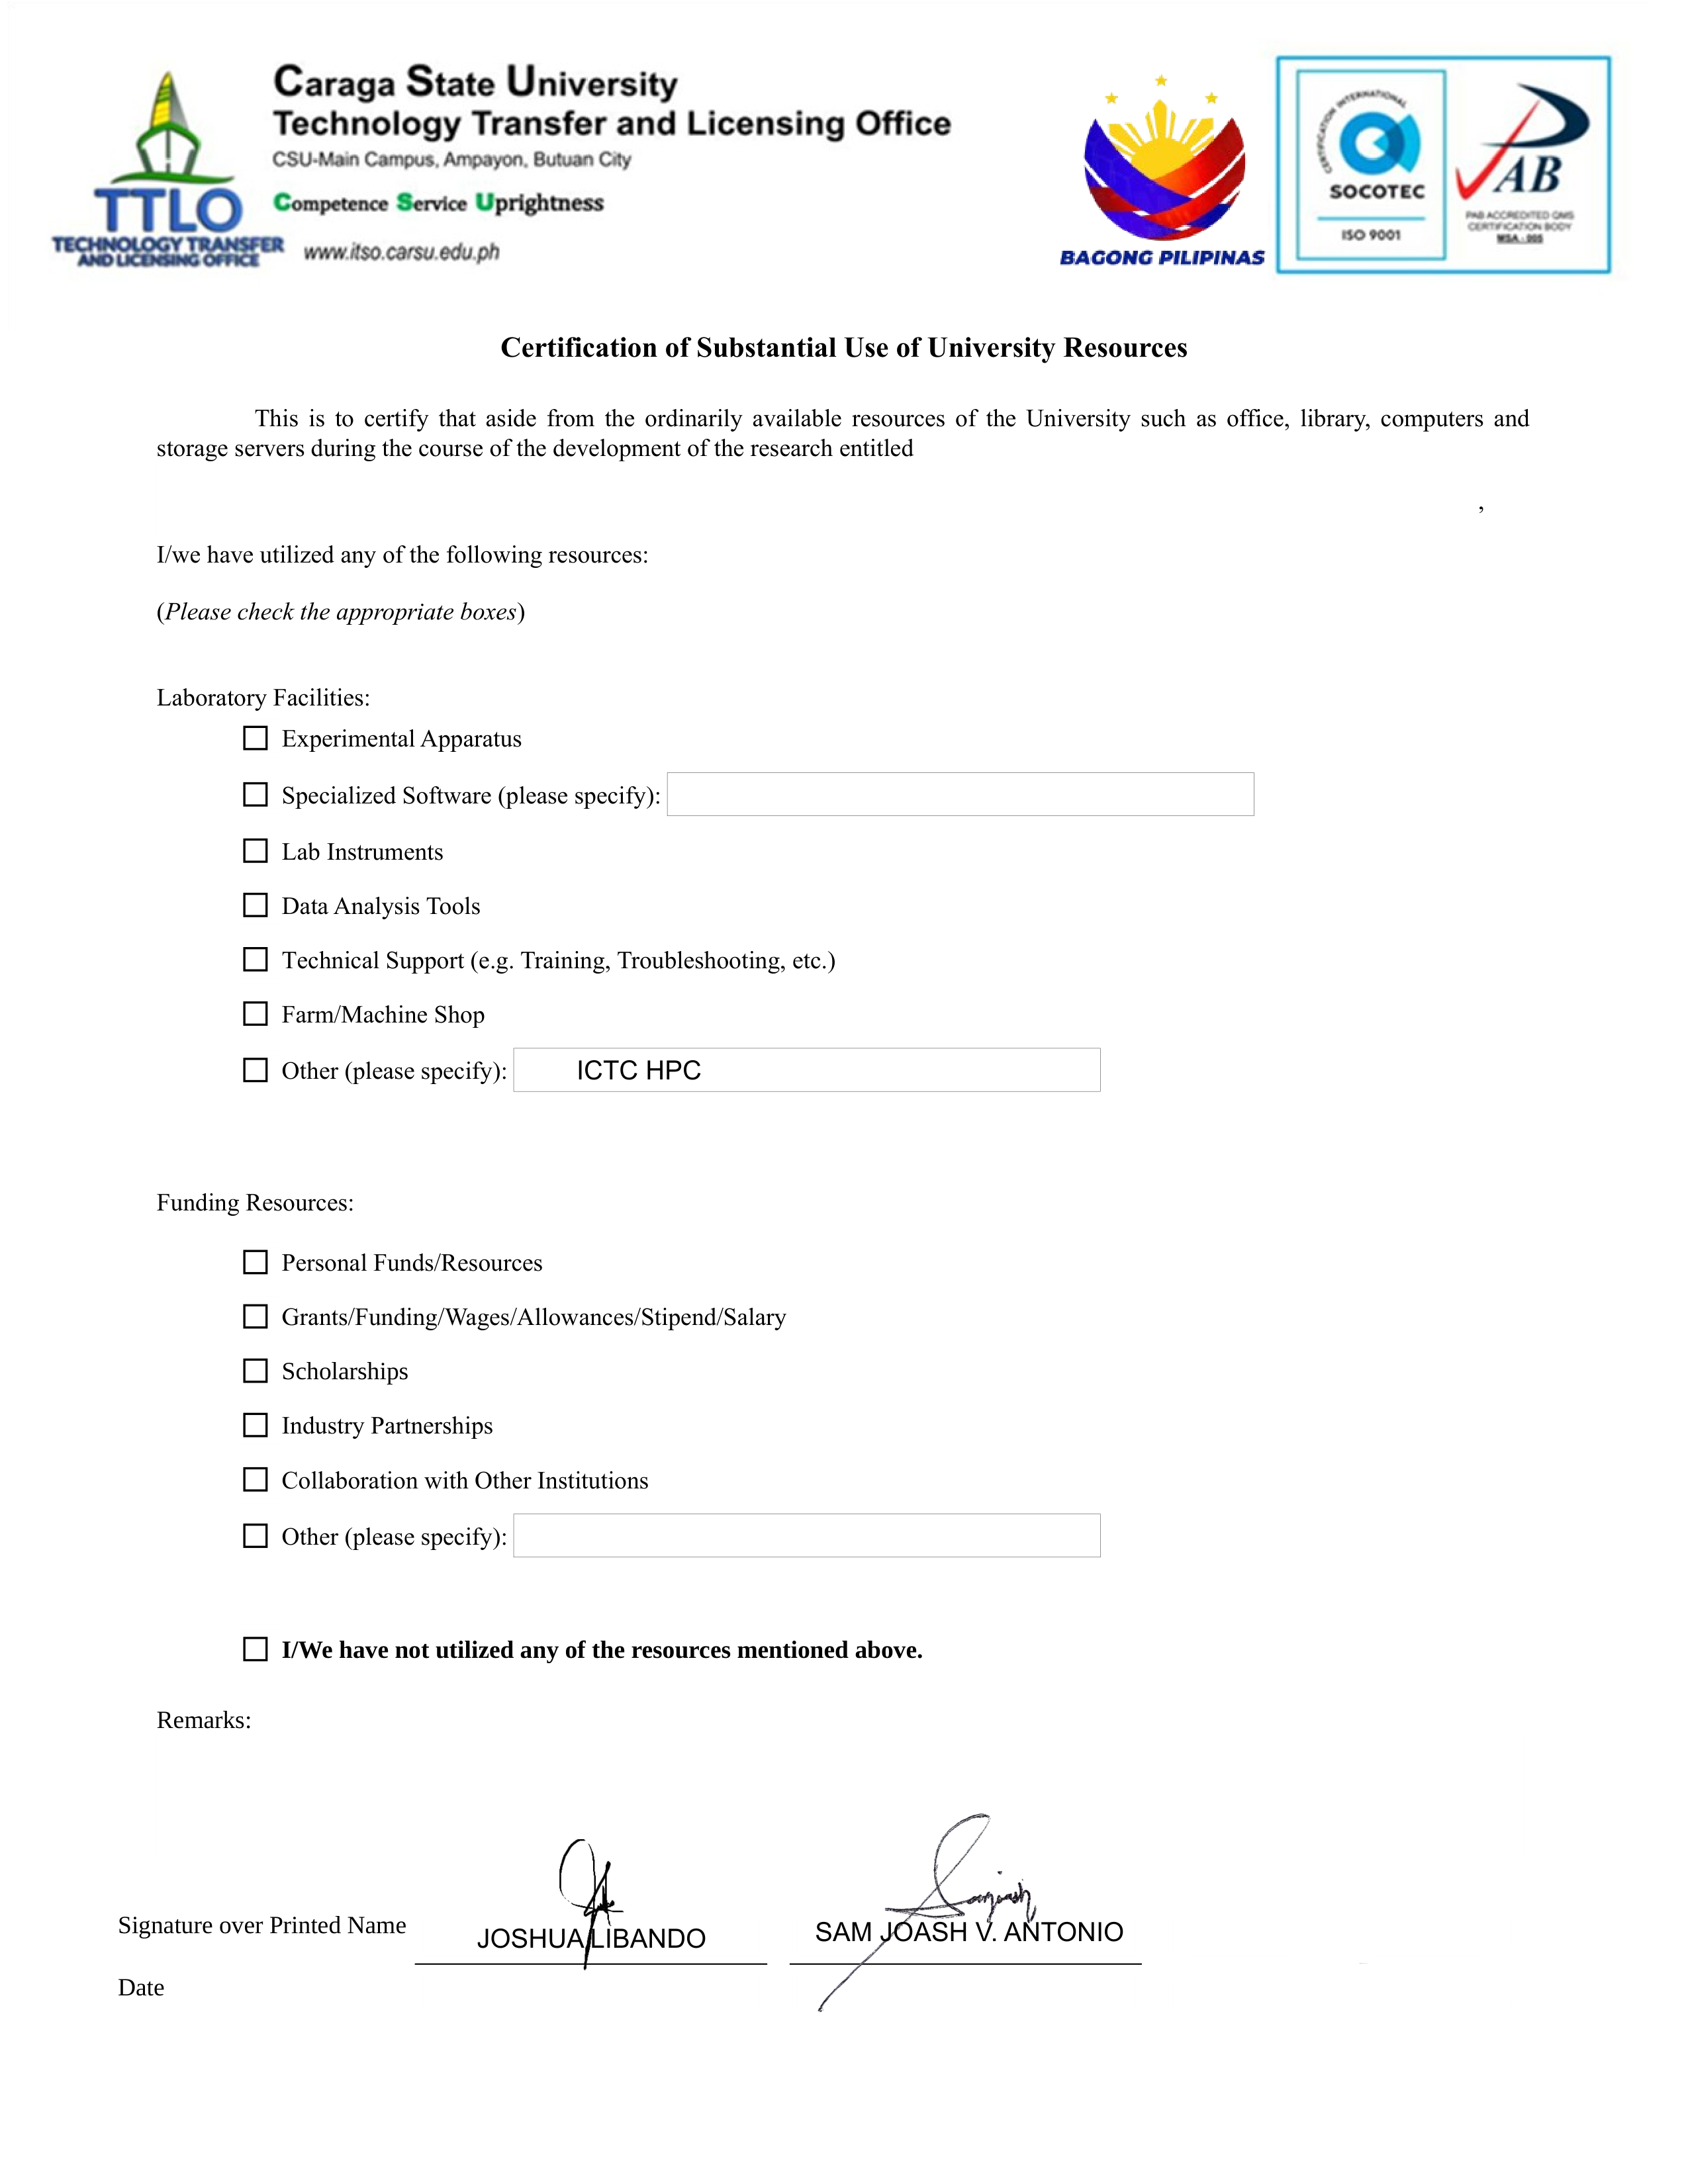
\includegraphics[
		width=\dimexpr\textwidth-2\fboxrule,
		height=0.85\textheight,
		keepaspectratio=true
		]{images/Certificate_of_substantial_use}}
\end{figure}
% \include{bionote}

\end{document}
\end{document}
